\documentclass[runningheads]{llncs}

\usepackage{graphicx}
\usepackage{url}
\usepackage{natbib}
\usepackage{lscape}
\usepackage{subfigure}
\usepackage{algorithm}
\usepackage{algorithmic}
\usepackage{setspace}
\usepackage{color}
\usepackage{tikz}
\usepackage{amssymb}
\usepackage{amsmath}


\urldef{\mailsg}\path|{rax222}@gmu.edu|
\newcommand{\keywords}[1]{\par\addvspace\baselineskip
\noindent\keywordname\enspace\ignorespaces#1}

\begin{document}


\mainmatter

\title{Simulating Financial Markets using MASON Framework\thanks{Prepared for the 2nd World Congress on Social Simulation, GMU, Fairfax, 14--17 July, 2008.}}

\titlerunning{Financial Markets using MASON}
\authorrunning{R. Axtell et al.}

\author{Robert Axtell$^{a}$ \and CSS 739 Class Project Team\thanks{Programming Group: Justin Briggs, Francesco Trusiano, Maciej \L atek, Randy Marks. Data Analysis Group: Sandler Lin, Cheryl Hansen and Thomas Tzitzouris.}}


\institute{
4400 University Drive, Fairfax VA 22030 \\
\mailss \\
\url{http://socialcomplexity.gmu.edu}}


\institute{$^{a}$Center for Social Complexity, George Mason University, USA \\
\mailsg}

\date{\today}
\maketitle

\keywords{Agent-based Modeling, Computational Social Science, Financial Markets}

\section{Motivation and Objectives}

The purpose of this project is to create computational platform that would be used to implement agent-based models of financial markets. In particular, following functionalities are desired:

\begin{itemize}
	\item Simulation may host heterogeneous agents that follow news processes, learn, obey budget constraints etc.;
	\item Many different assets traded on markets using different trading rules may be present (based on price-impact heuristics, double auction);
	\item Flexible GUI and reporting facilities, including ability to summarize batch results from sensitivity analysis.
\end{itemize}

This paper outlines the prototype prepared during the CSS739 class, presents three sample models and follows the steps taken to ensure correctness of our implementation. 

\section{Platform Architecture}

The implementation took place using MASON simulation framework, see \cite{luke2005}. The static structure of our platform is outlined on Figure \ref{fig:general_class}, where UML class diagram is presented (minus classes corresponding to orders). Figure \ref{fig:general_sequence} presents interactions taking place during a sample iteration between two agents and an orderbook.  

\begin{figure}[htb]
\centering
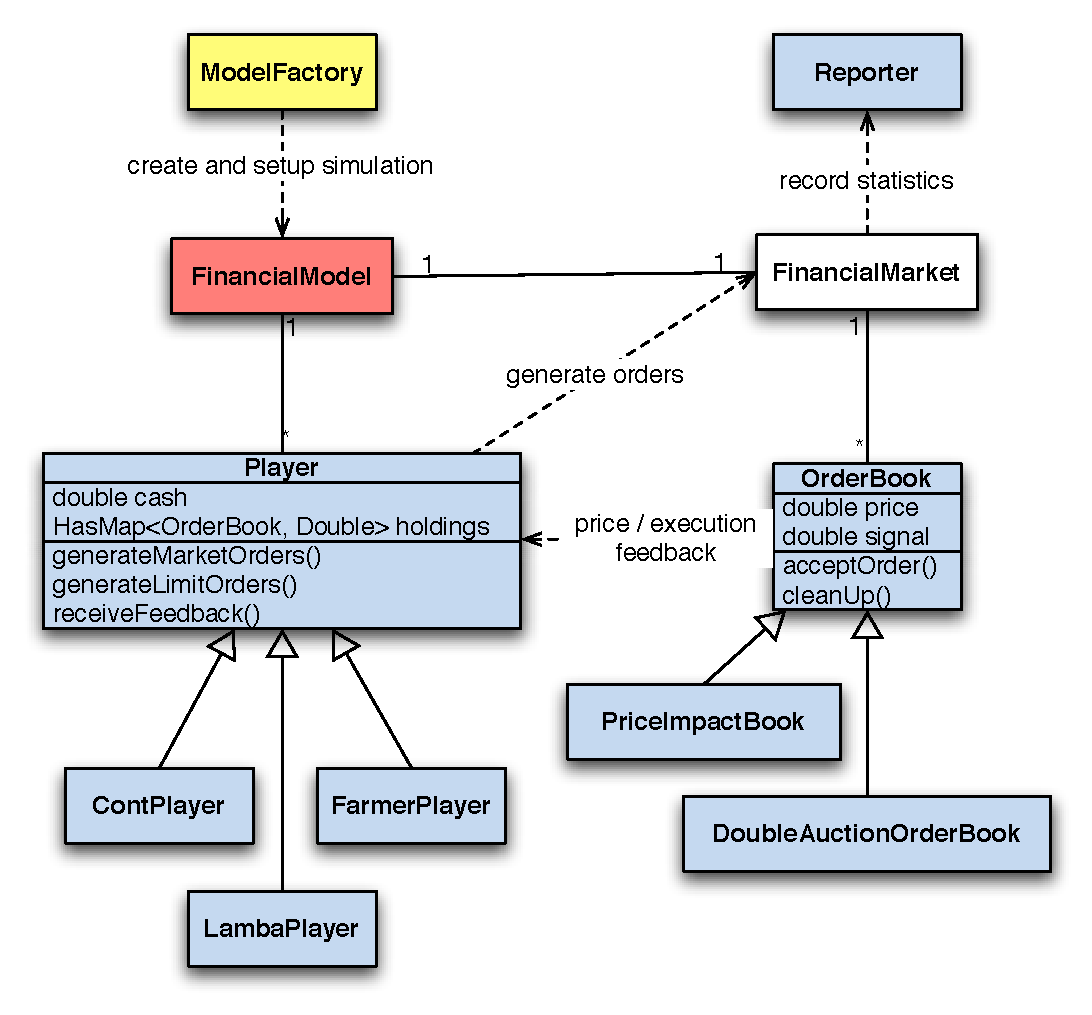
\includegraphics[width=1.0\textwidth]{../graphics/masterClassDiagram.pdf}
\caption{High-level UML class diagram of the main components and relations in the FinancialMarketModel, including the main attributes of Players and OrderBooks. Agent classes (light blue) inherit from the MASON \texttt{Steppable} interface while the master class is implementation of MASON's \texttt{SimState}.}
\label{fig:general_class}
\end{figure}

\begin{figure}[htb]
\centering
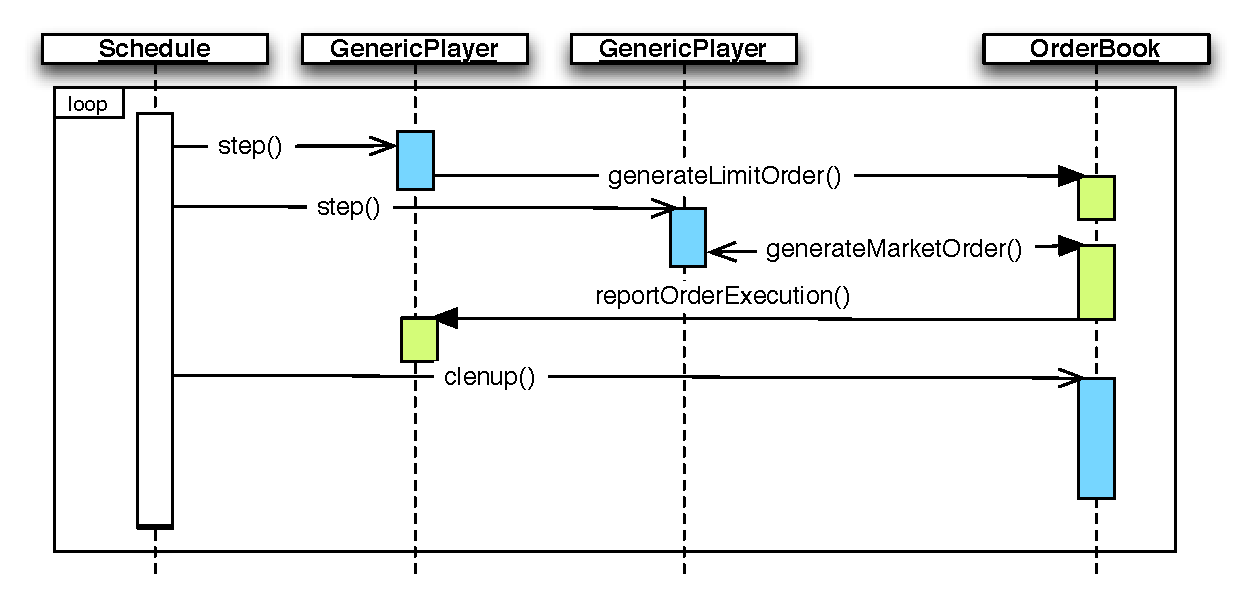
\includegraphics[width=1.0\textwidth]{../graphics/masterSequenceDiagram.pdf}
\caption{High-level UML sequence diagram of the interactions between main object of the FinancialMarketModel, with messages send between two agents and a single orderbook during a single tick shown. Agents are activated by MASON simulation engine and may generate different kinds of \texttt{Market}- and \texttt{LimitOrders}, depending on their internal states and signals from environment (prices, news process). The \texttt{MarketOrder} gives an agent instantaneous feedback, whereupon effects of LimitOrder may be delayed in time. The \texttt{cleanup} signal causes the Orderbook to arbitrage all possible trades between \texttt{LimitOrders}, recalculate new prices and returns (if applicable) and remove expired orders.}
\label{fig:general_sequence}
\end{figure}


\section{Implemented Models}

\subsection{Cont Model}

The Cont model (\cite{cont2006}) is the simplest model implemented. All traders (agents) follow the same behavioral rules. They are heterogeneous in the sense that they are given independently assigned (subjective) volatility thresholds $\theta_i(t)$. Each period, all agents receive a common signal, which can be interpreted as public information or "news", in the form of IID Gaussian random variables $\epsilon_t ~ N(0,D^2)$. Each agent $i$ responds to this signal by selling if $\epsilon_t < -\theta_i(t)$, buying if $\epsilon_t > \theta_i(t)$, and otherwise sitting out the period. The market then determines the excess demand and arrives at the market clearing price by means of a market impact function. Lastly, with probability $s$, agents update their threshold to match the absolute value of the return rate for the current period. Somewhat surprisingly, even this very simple "zero intelligence" model of agent behavior yields fairly realistic market movements, as presented in Figures \ref{fig:ContSmallSSim} (for small $s$) and \ref{fig:ContLargeSSim} (for large value of $s$). 

\paragraph*{}
One down side of the Cont model that is not noted in the papers is that there appears to be a great degree of periodic cyclicality in the volatility of the markets. This is especially apparent with higher probability $s$ of updating thresholds. With $s=0.1$, this is readily apparent if you look at the autocorrelation of absolute returns over longer time scales than shown in the paper. This effect can be particularly well seen when averaging over many runs, as on Figure \ref{fig:ContMultiRun}. Holding $s$ constant at $0.1$ and varying $D$, we find the period and amplitude to be predictable.

\begin{figure}[htbp]
  \begin{center}
   \mbox{
    \subfigure[Trade volumes.]{\scalebox{0.33}{ 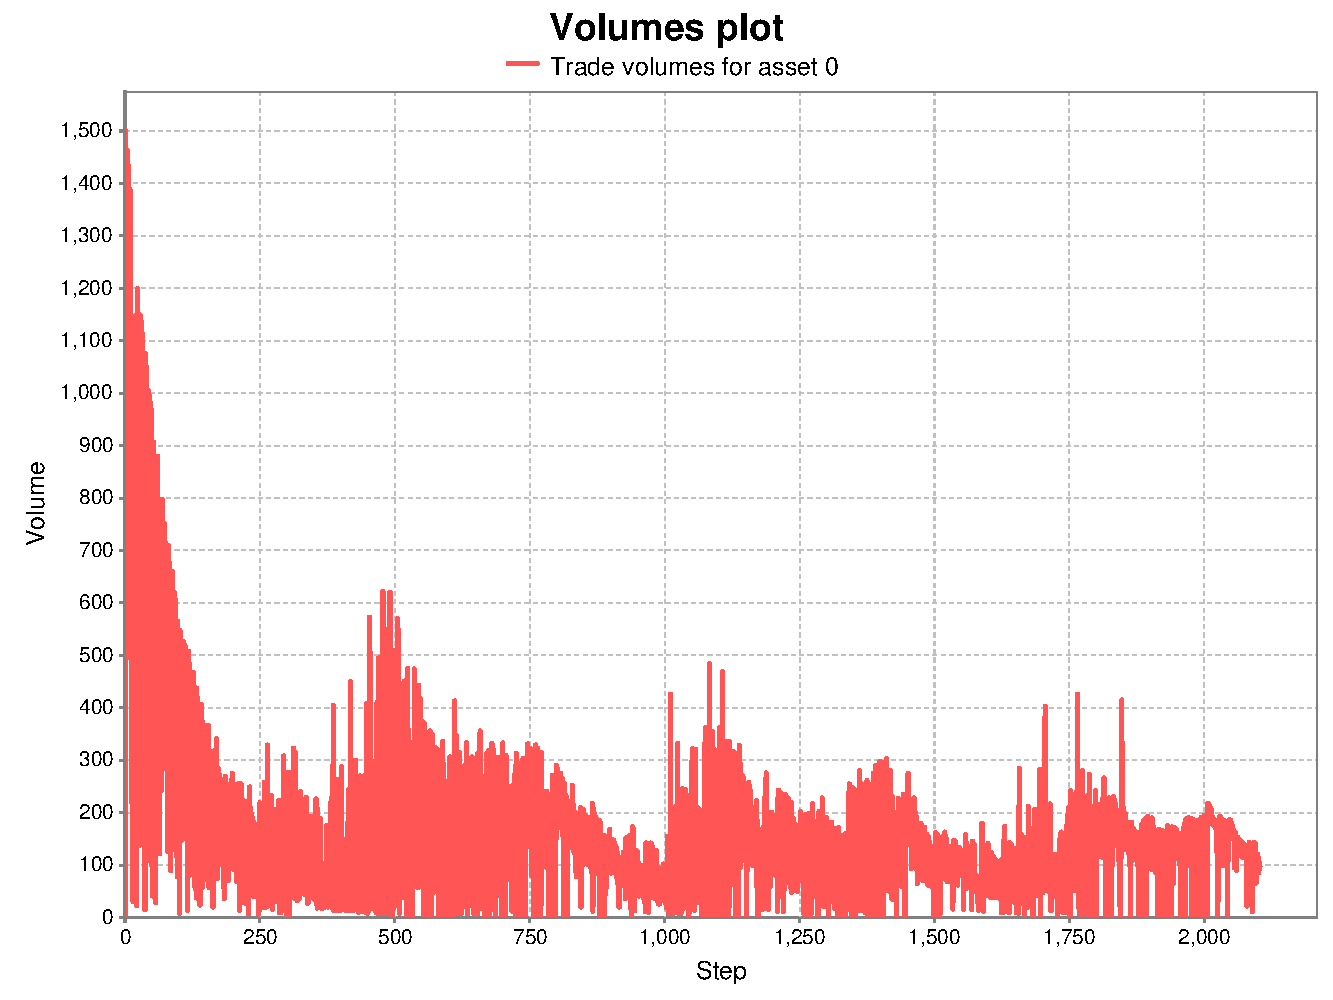
\includegraphics[width=1.00\textwidth]{../graphics/Cont-s01-volumesPlot.pdf}}}
    \quad
\subfigure[Price]{\scalebox{0.33}{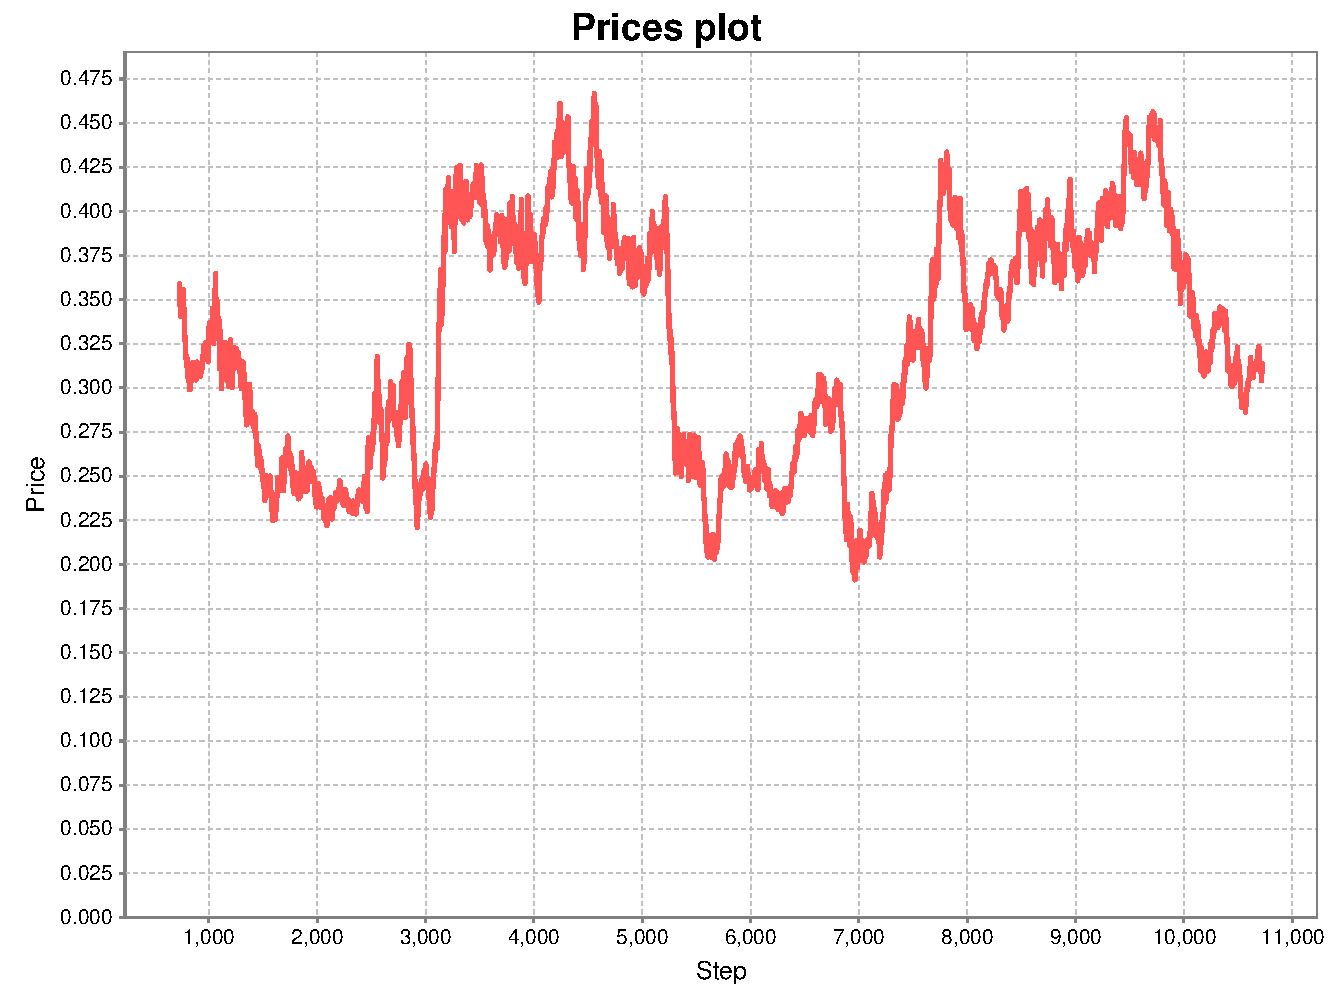
\includegraphics[width=1.0\textwidth]{../graphics/Cont-s01-pricesPlot.pdf}}}
}
    \mbox{
      \subfigure[Raw and absolute log returns.]{\scalebox{0.33}{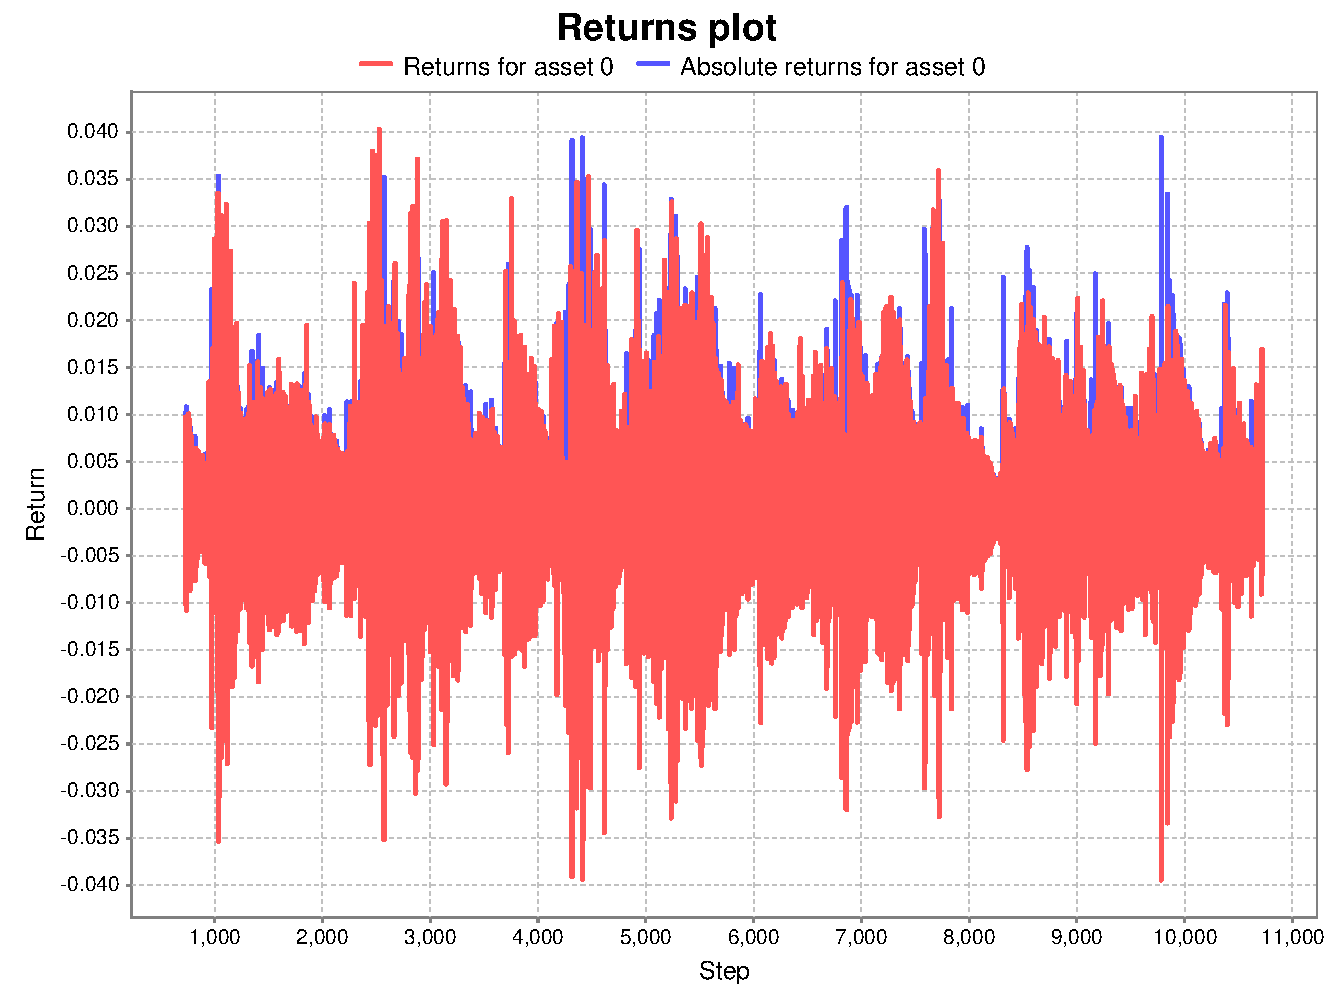
\includegraphics[width=1.00\textwidth]{../graphics/Cont-s01-returnsPlot.pdf}}}
      \quad
      \subfigure[Distribution of Returns]{\scalebox{0.33}{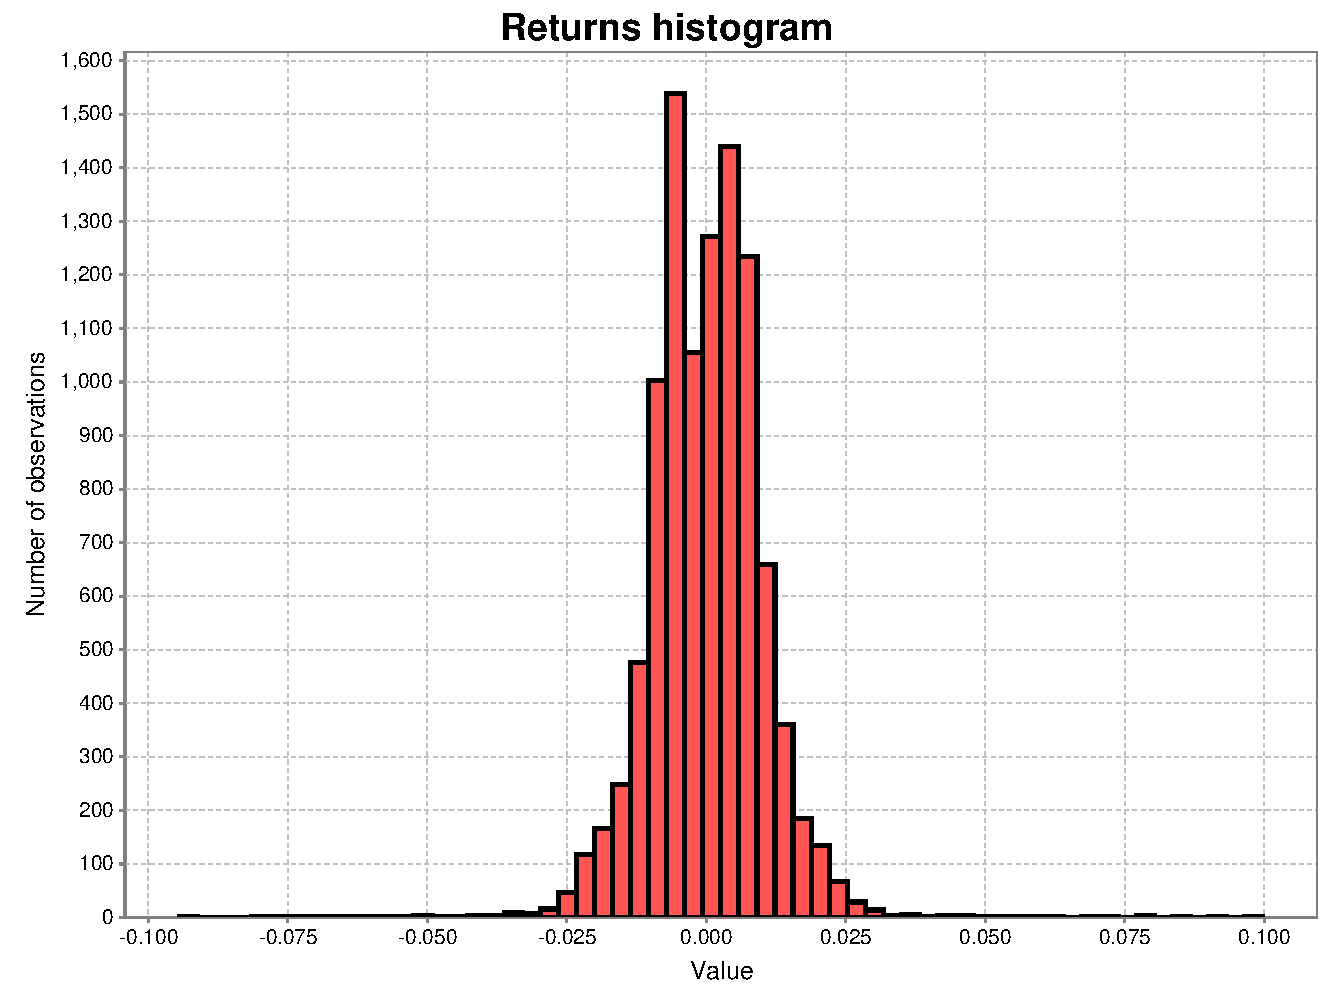
\includegraphics[width=1.00\textwidth]{../graphics/Cont-s01-returnsHistogram.pdf}}}       
      \quad
      \subfigure[Distribution of Returns (log scale)]{\scalebox{0.33}{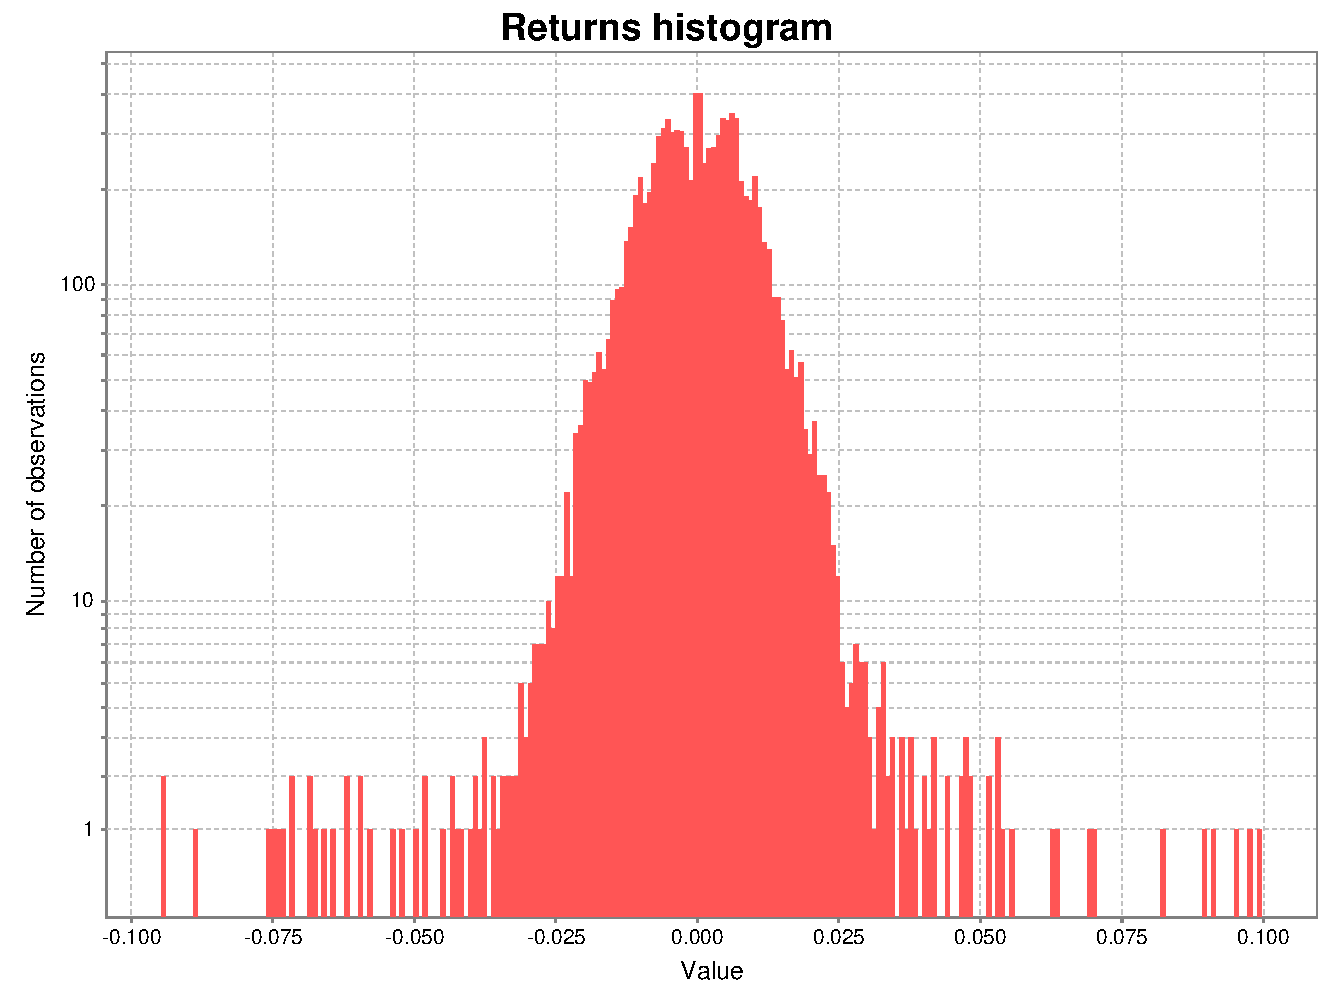
\includegraphics[width=1.00\textwidth]{../graphics/Cont-s01-logReturnsHistogram.pdf}}}       
}
    \mbox{
      \subfigure[Annualized moving average volatility]{\scalebox{0.33}{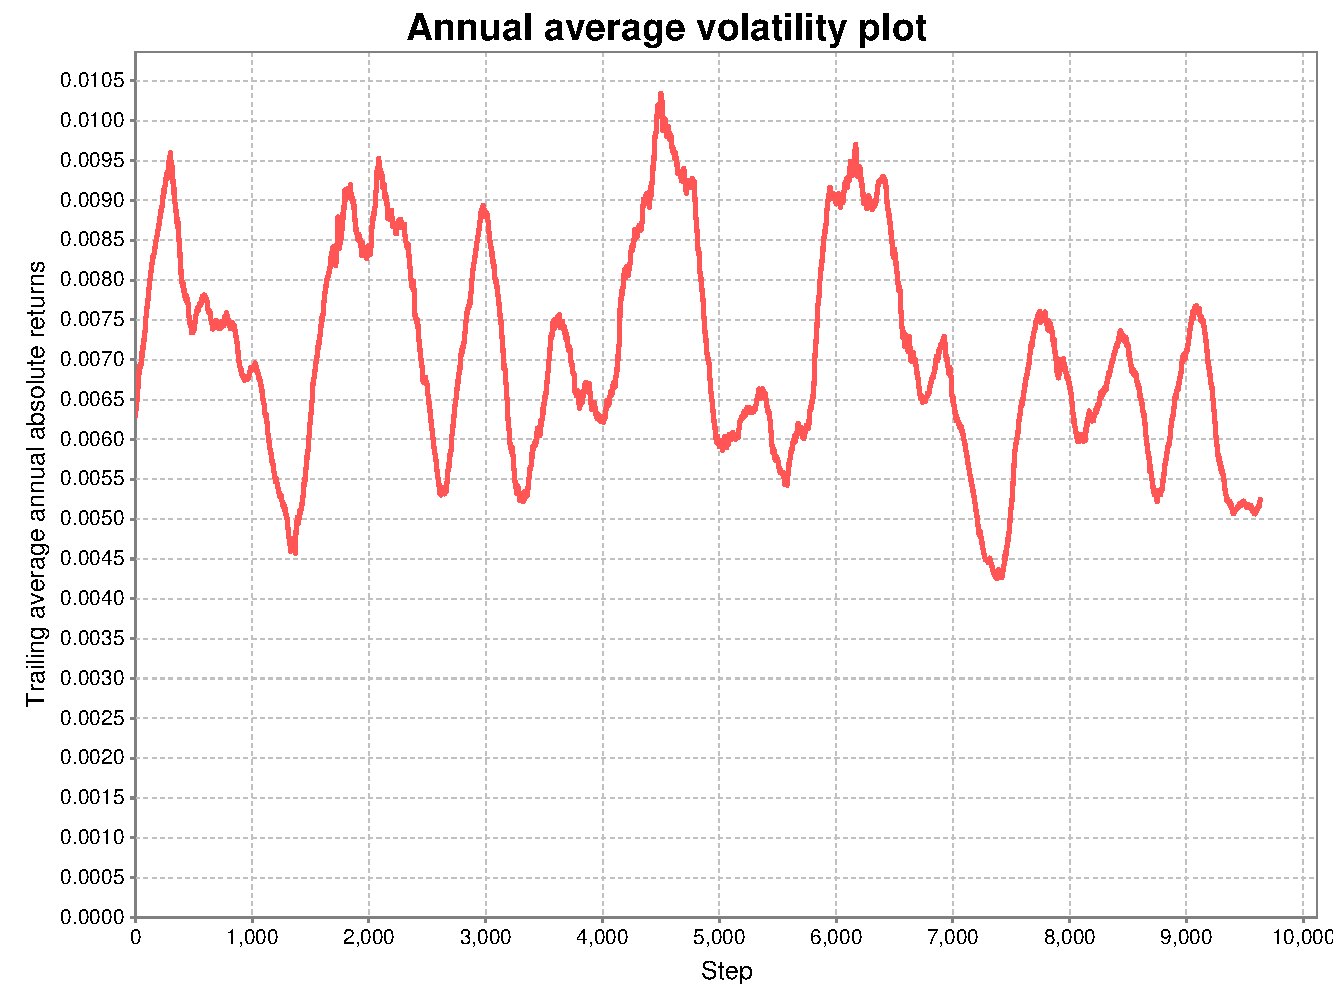
\includegraphics[width=1.00\textwidth]{../graphics/Cont-s01-avgVolatility.pdf}}}
      \quad
      \subfigure[Autocorrelation of returns.]{\scalebox{0.33}{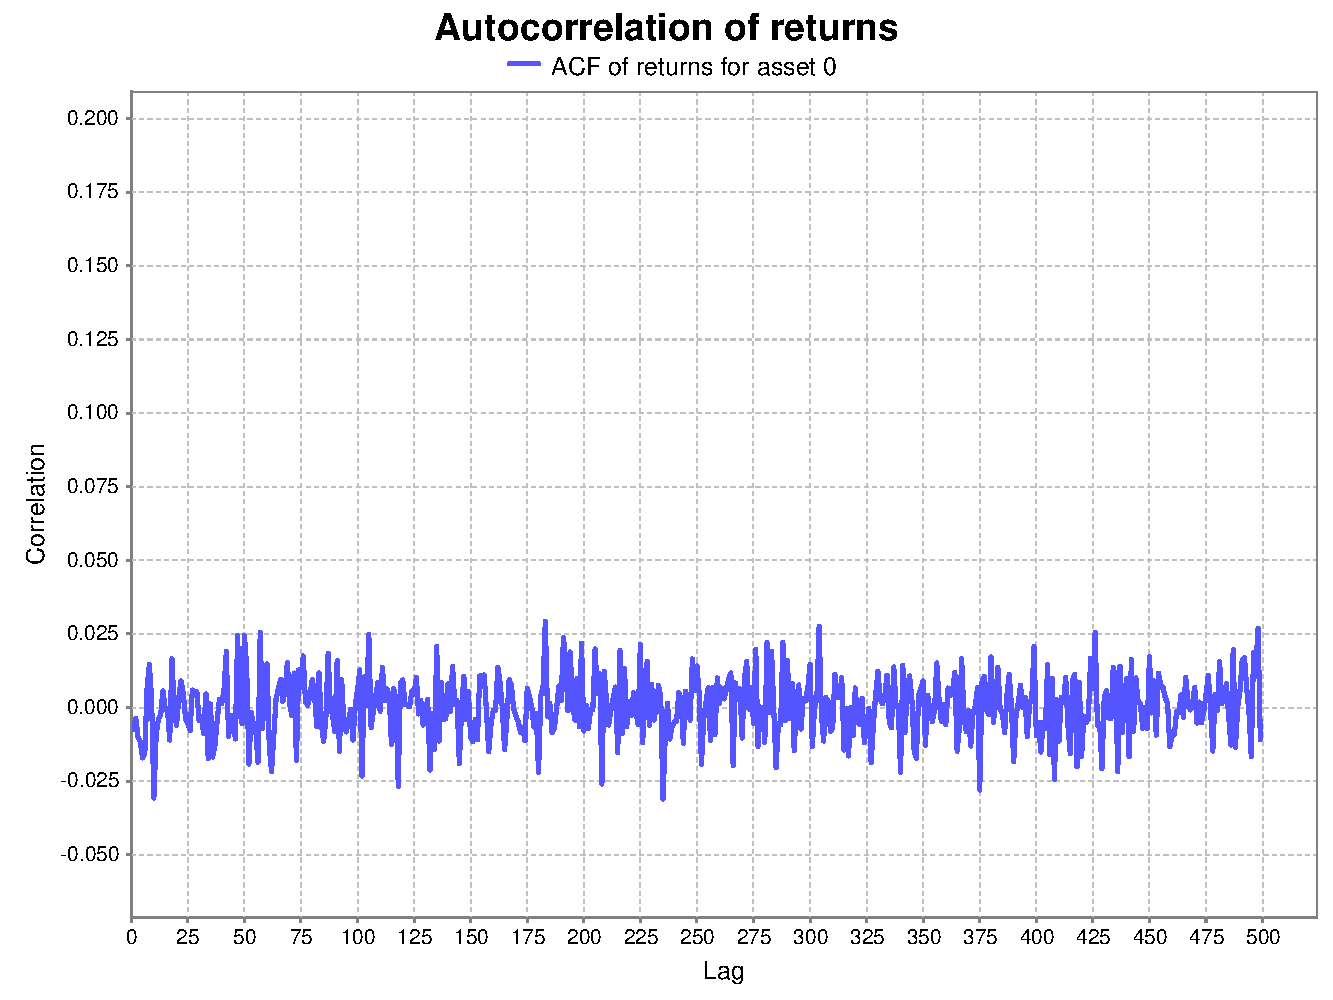
\includegraphics[width=1.00\textwidth]{../graphics/Cont-s01-acfPlot-noAbs.pdf}}}
      \quad
      \subfigure[Autocorrelation of absolute returns.]{\scalebox{0.33}{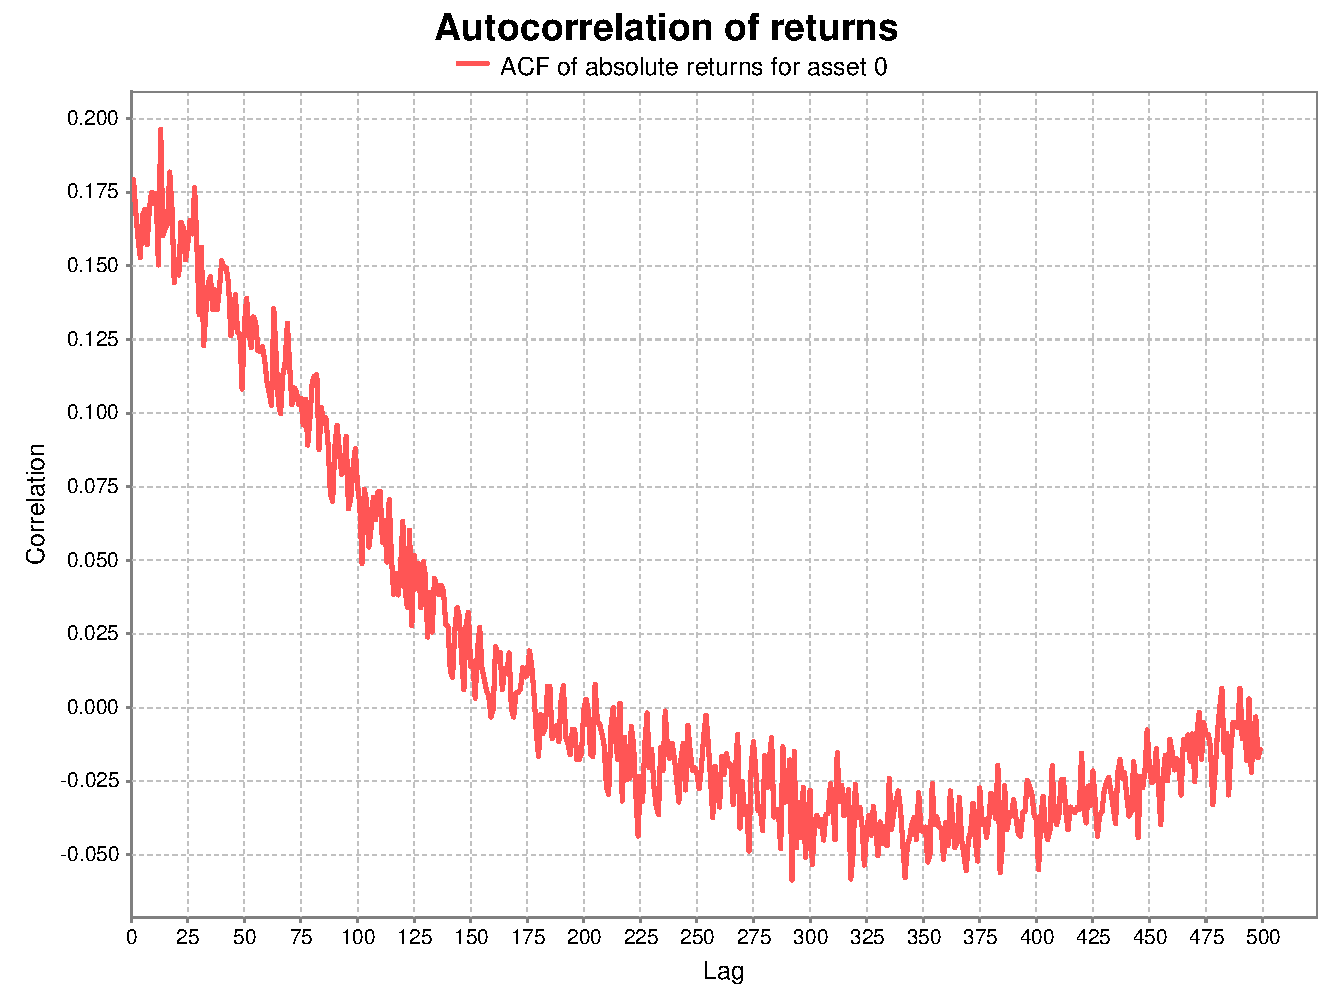
\includegraphics[width=1.00\textwidth]{../graphics/Cont-s01-acfPlot-absonly.pdf}}}
      }
    \caption{Examples of outputs and statistics from a single run of the Cont FinancialModel simulation with $D=0.001$, $s=0.01$.}
    \label{fig:ContSmallSSim}
  \end{center}
\end{figure}




\begin{figure}[htbp]
  \begin{center}
   \mbox{
      \subfigure[Trade volumes.]{\scalebox{0.33}{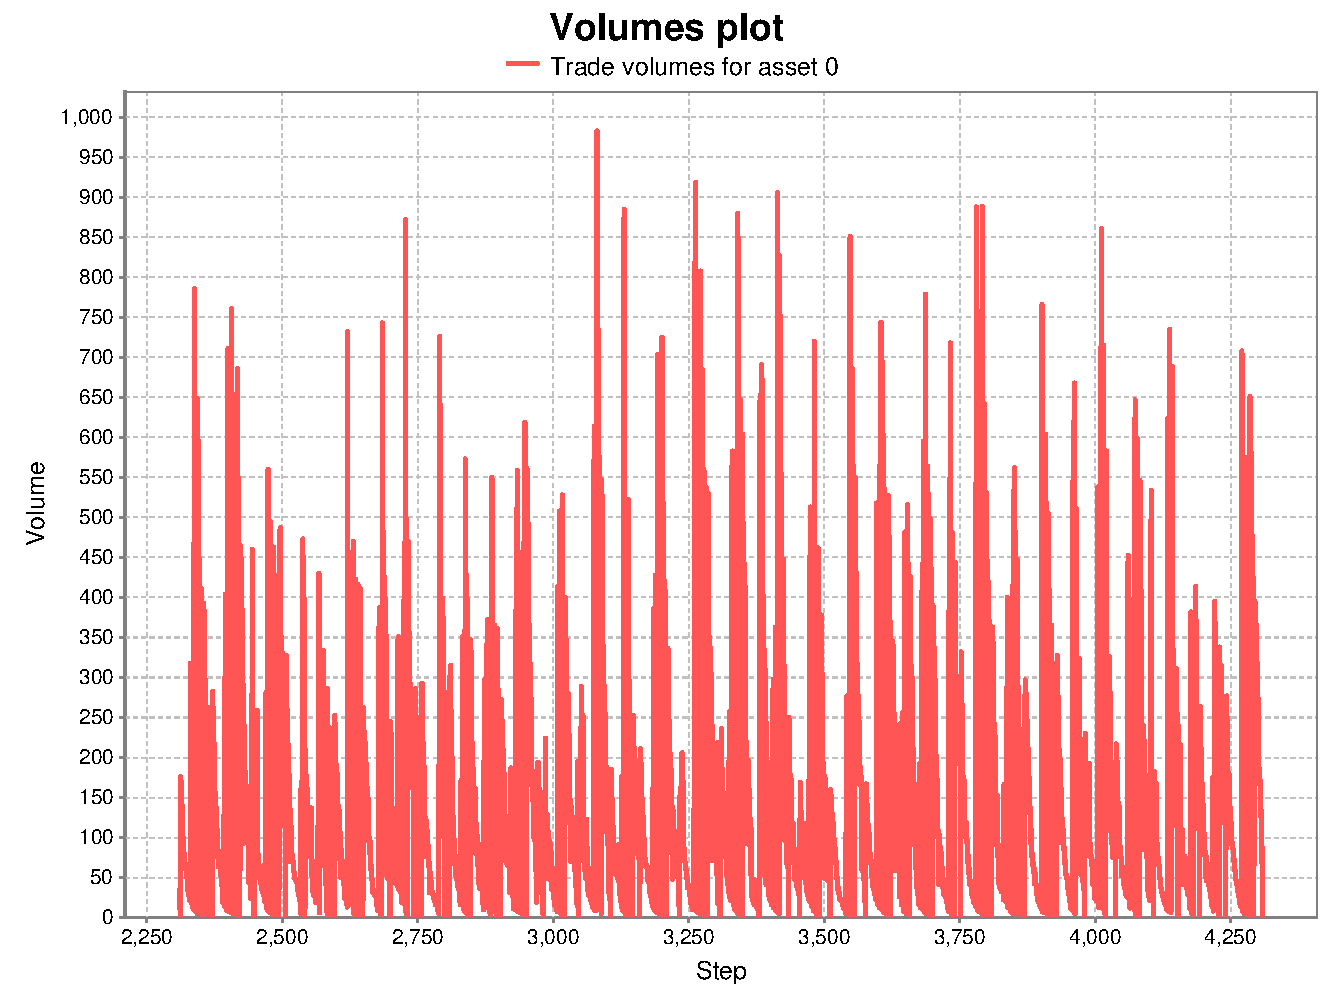
\includegraphics[width=1.00\textwidth]{../graphics/Cont-volumesPlot.pdf}}}
      \quad
      \subfigure[Price]{\scalebox{0.33}{ 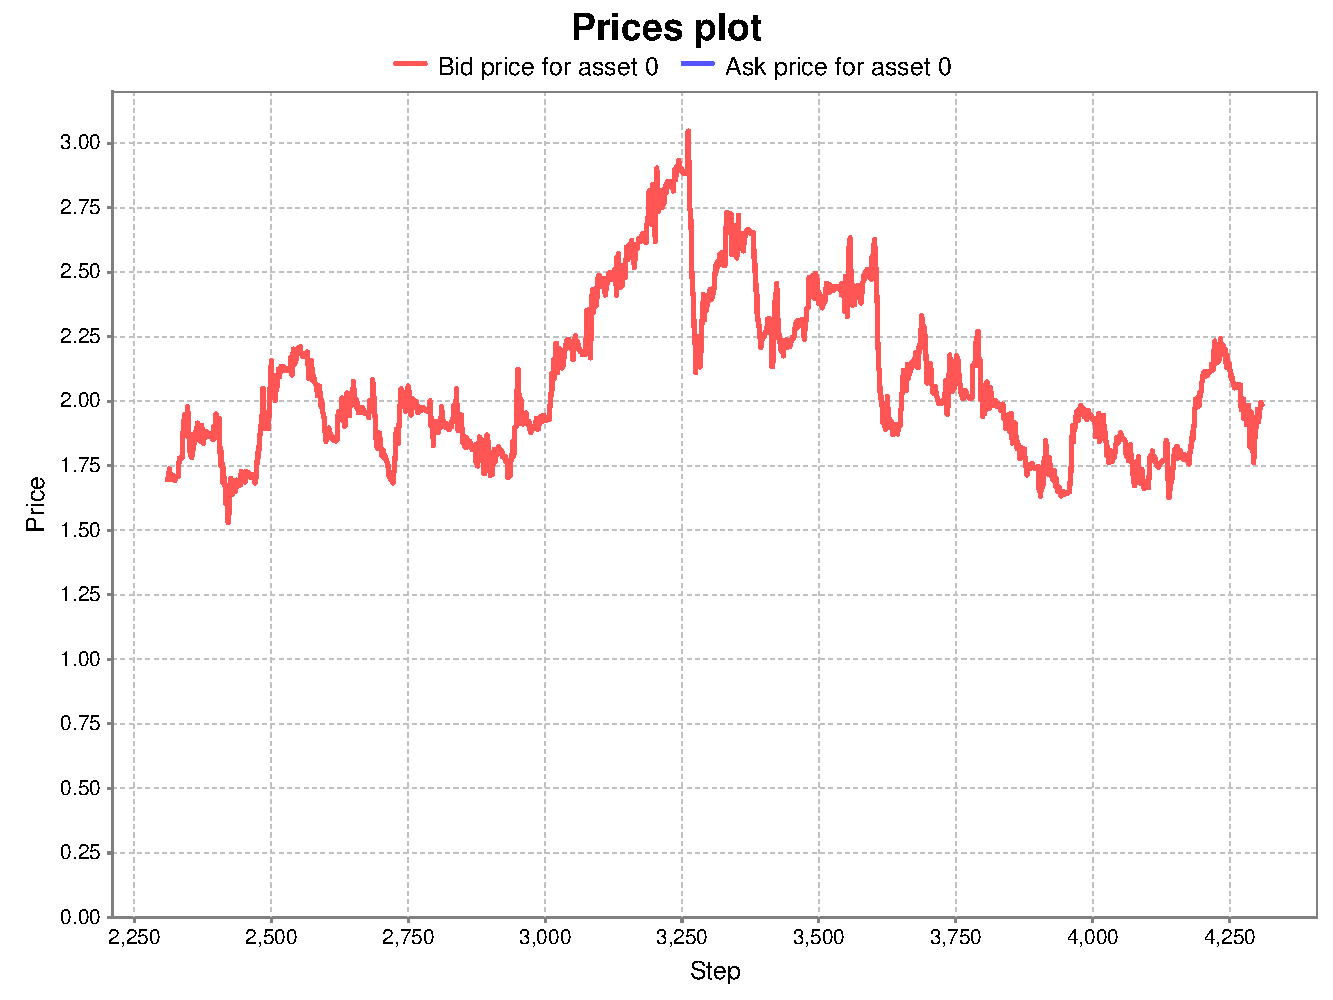
\includegraphics[width=1.0\textwidth]{../graphics/Cont-pricesPlot.pdf}}} \quad
      }
    \mbox{
      \subfigure[Raw and absolute log returns.]{\scalebox{0.33}{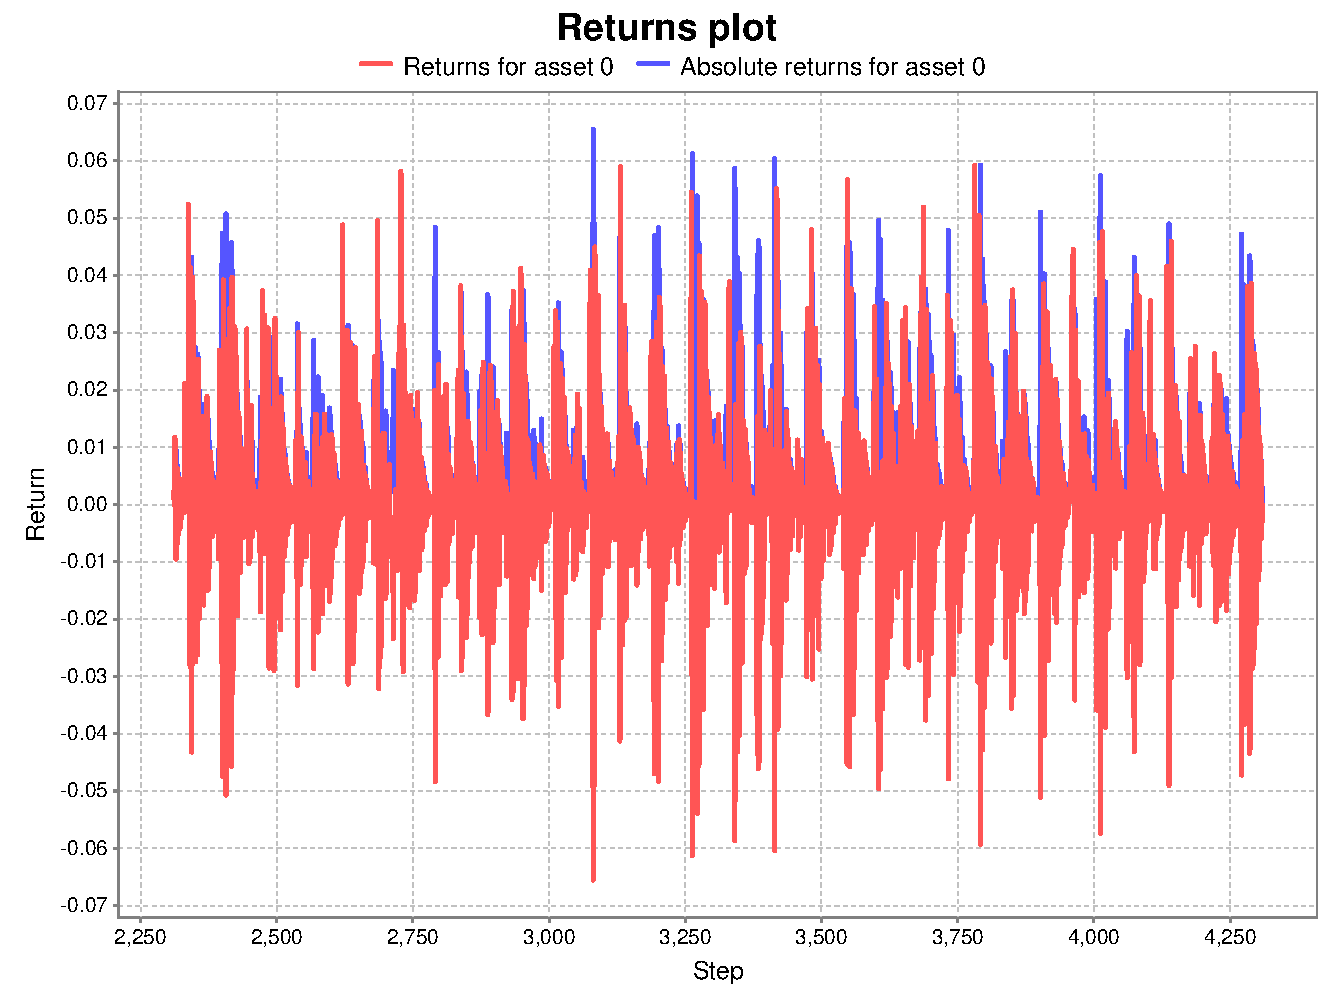
\includegraphics[width=1.00\textwidth]{../graphics/Cont-returnsPlot.pdf}}}
      \quad
      \subfigure[Returns histogram.]{\scalebox{0.33}{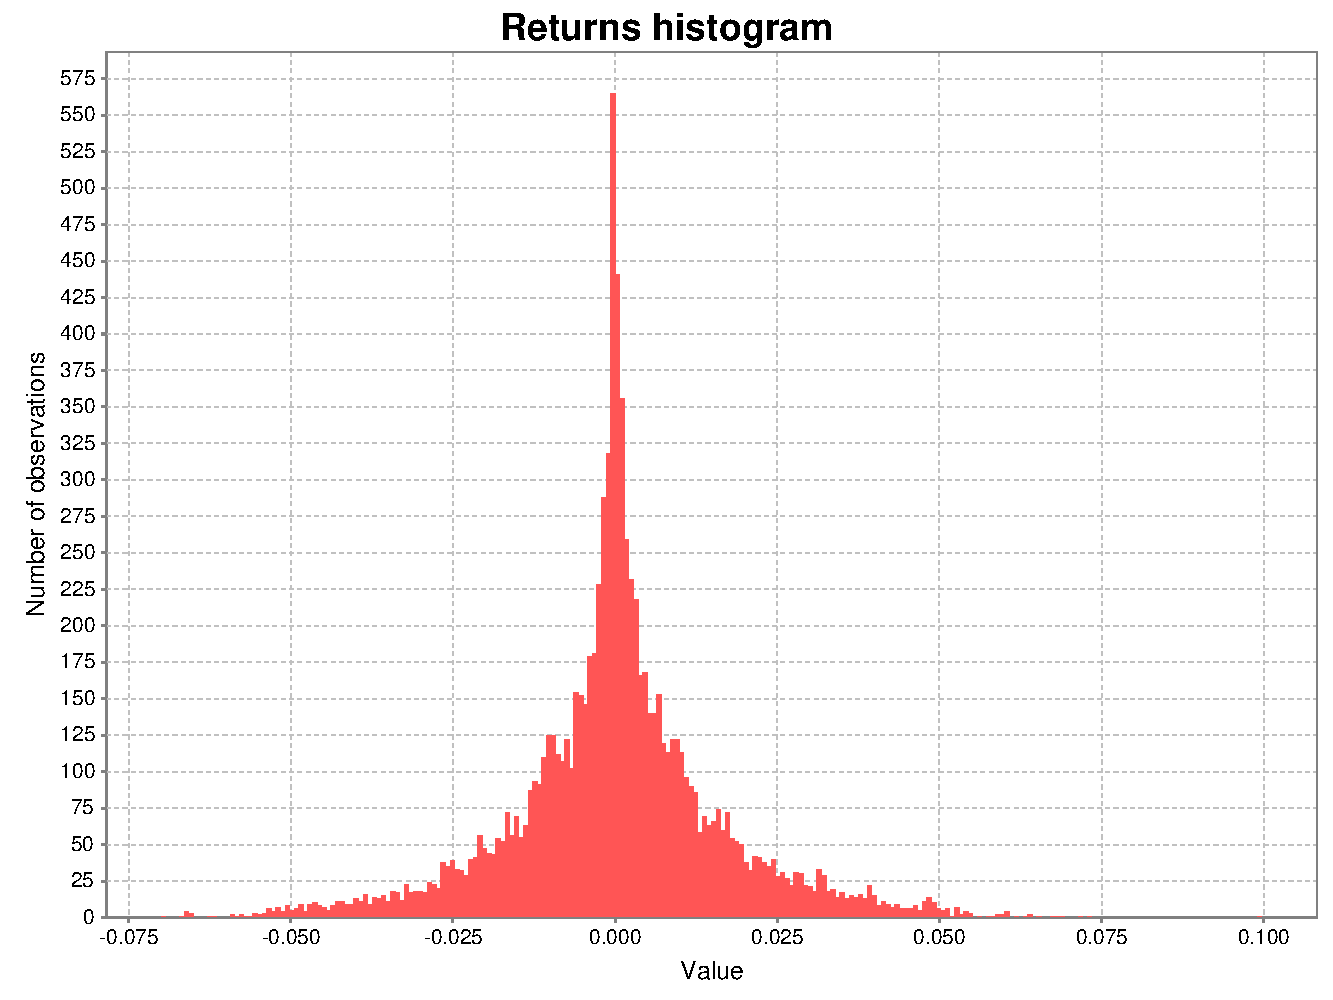
\includegraphics[width=1.00\textwidth]{../graphics/Cont-returnsHistogram.pdf}}}
      \quad
      \subfigure[Distribution of Returns (log scale)]{\scalebox{0.33}{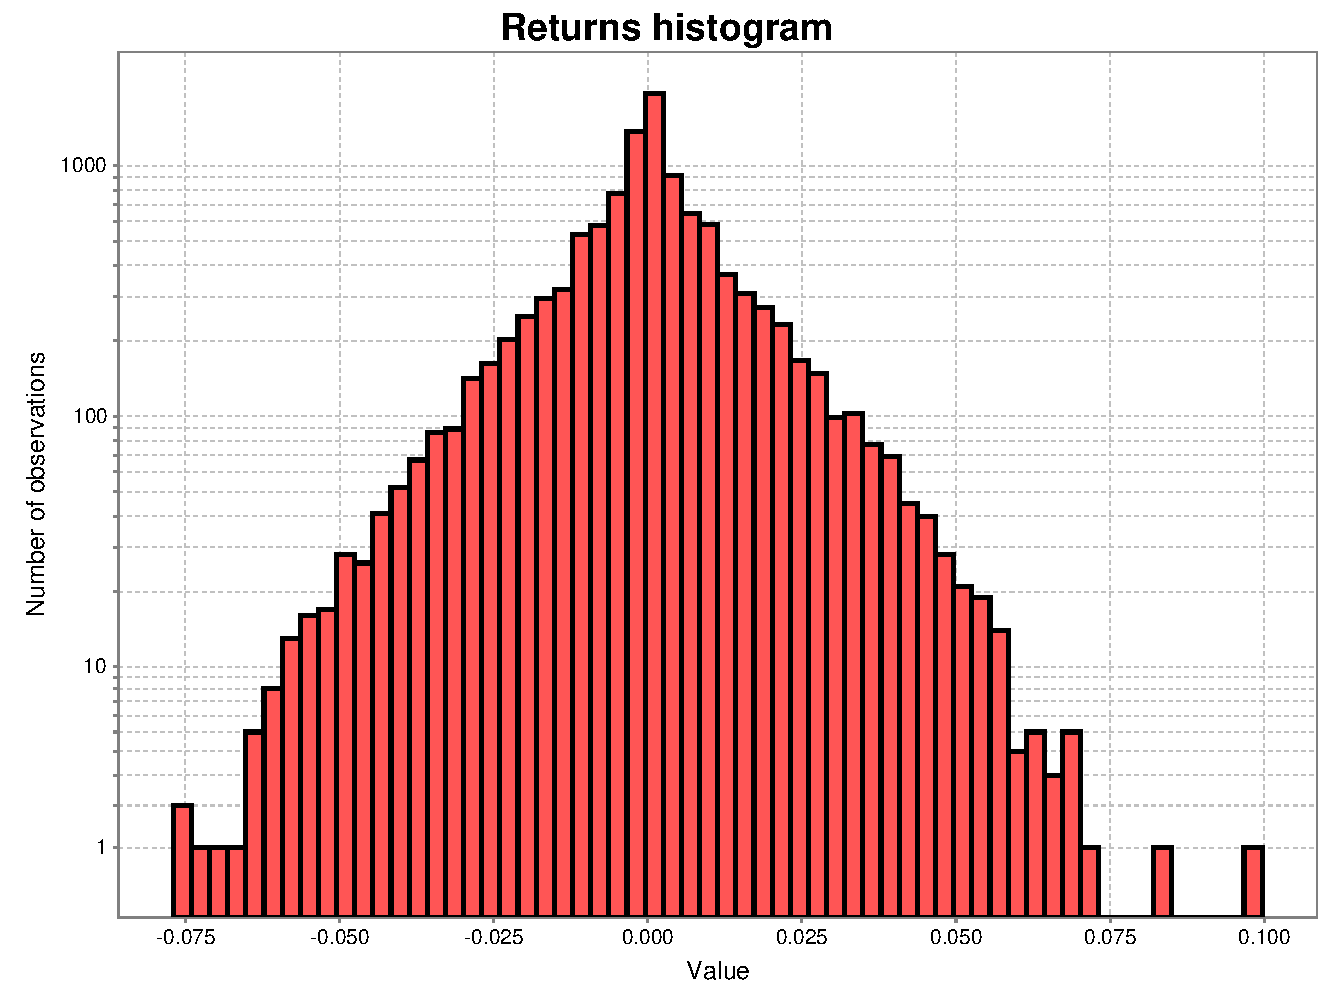
\includegraphics[width=1.00\textwidth]{../graphics/Cont-logReturnsHistogram.pdf}}}       
}
    \mbox{
      \subfigure[Annualized moving average volatility]{\scalebox{0.33}{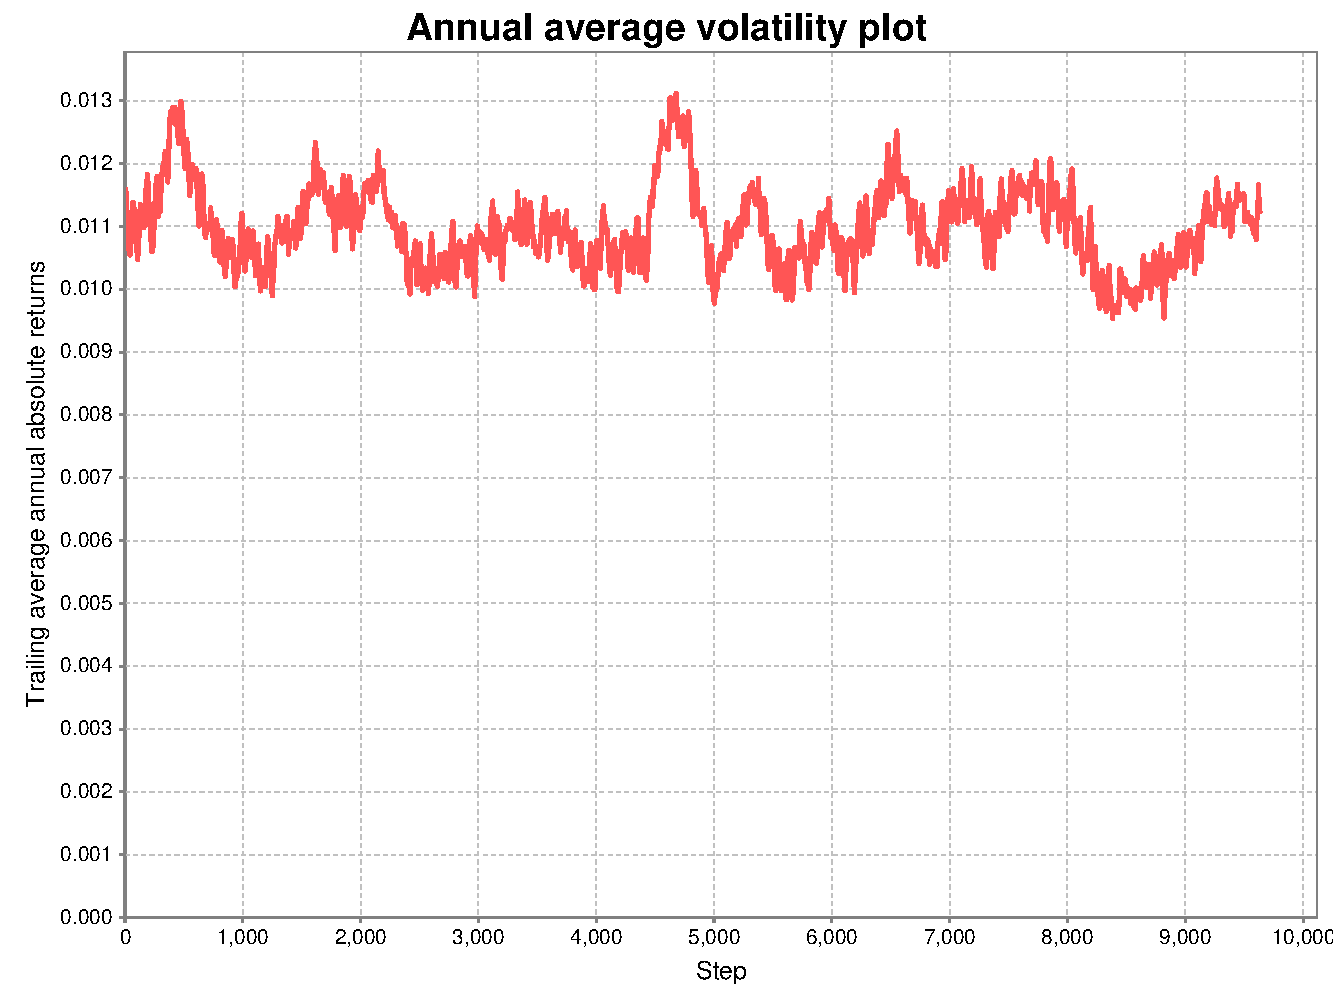
\includegraphics[width=1.00\textwidth]{../graphics/Cont-avgVolatility.pdf}}}
      \quad
      \subfigure[Autocorrelation of returns.]{\scalebox{0.33}{\includegraphics[width=1.00\textwidth]{../graphics/Cont-acfPlot-noAbs.pdf}}}
      \quad
      \subfigure[Autocorrelation of absolute returns.]{\scalebox{0.33}{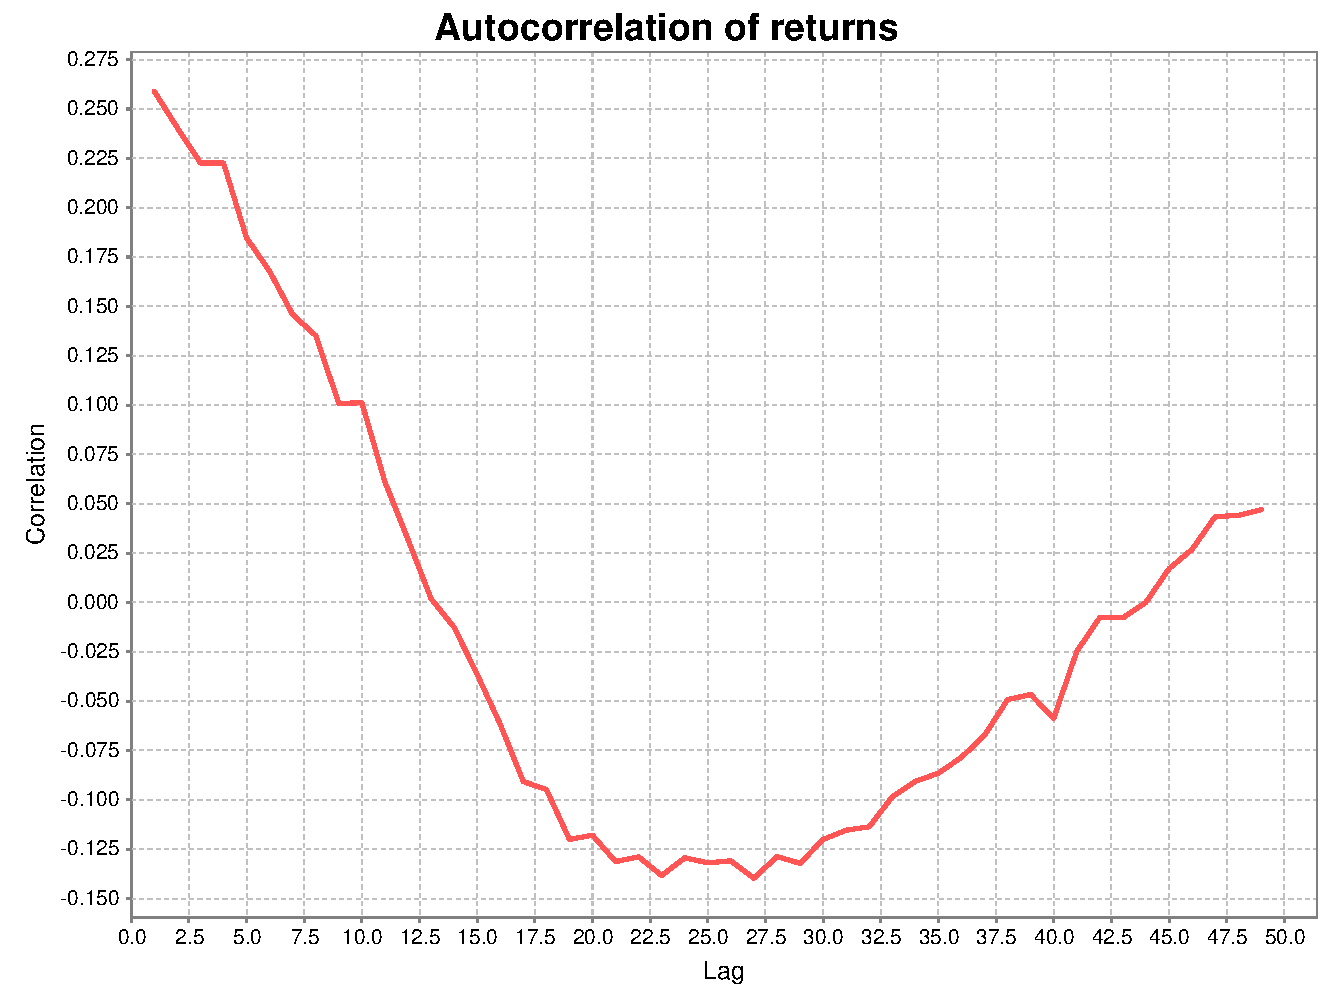
\includegraphics[width=1.00\textwidth]{../graphics/Cont-acfPlot-absonly-to50.pdf}}}
      }
    \caption{Examples of outputs and statistics from a single run of the Cont FinancialModel simulation with $D=0.001$, $s=0.1$.}
    \label{fig:ContLargeSSim}
  \end{center}
\end{figure}


\subsection{Farmer Model}

The Farmer model (\cite{farmer2003}) has two types of agents, which trade a single asset by means of a continuous double auction similar to those normally used on stock markets. "Patient" traders place limit orders, which specify both a price and quantity they wish to buy or sell. Limit orders do not execute immediately, and may be canceled at any time. "Impatient" traders place market orders, specifying only a quantity, which execute immediately at the current best price, assuming there is sufficient liquidity provided by outstanding limit orders. This model also has simple behavioral logic for traders. Behavior is regulated by:
\begin{itemize}
\item Patient agents place \texttt{LimitOrders} of constant size $\sigma$ at a Poisson rate of $\alpha$ per unit time, and with a randomly generated price. Orders are equally likely to be either buy or sell orders. Buy limit orders are placed uniformly anywhere in the semi-infinite interval below the current ask price ($-\infty < p < a(t)$), where $p$ is the \emph{logarithm} of the price; similarly for sell orders. A uniform distribution in log prices is equivalent to an exponential distribution in prices. In addition, outstanding limit orders are cancelled at a Poisson rate of $\delta$ per unit time. All of these processes are independent.
\item Impatient agents place \texttt{MarketOrders} of constant size $\sigma$ at a Poisson rate of $\mu$ per unit time.
\item A double auction order book. This manages the pending limit orders and facilitates trades between market and limit orders. It also provides aggregate market information such as return rate per unit time and bid-ask spreads.
\end{itemize}
\paragraph*{}
This model explains a large portion of the spread and price diffusion of actual stocks given an order flow rate, which implies that the double auction structure has a significant impact on the nature of market movements. The model also yields market behavior qualitatively close to actual markets in many respects, see Figure \ref{fig:sampleDynamicsFarmer}.
\paragraph*{}
However, as a model of market dynamics, it fails on some fronts. Notably, we do not see realistic volatility clustering. Volumes are fairly consistent, as are average returns. There is no lingering positive autocorrelation of absolute returns. Also notice the amplitude of single-period returns in Figure \ref{fig:sampleDynamicsFarmer}(g). The average per-step absolute returns are around $20\%$, much higher than empirically plausible, at least if a step is meant to signify short period, such as a day or less. This is clearly seen when we use actual prices in the order book. The same prices which look somewhat reasonable when viewed on a log scale appear quite volatile prices when viewed on a normal scale as in Figure \ref{fig:dynamicsFarmerNonLog}.

\begin{figure}[htbp]
  \begin{center}
   \mbox{
      \subfigure[Snapshot of Orderbook.]{\scalebox{0.5}{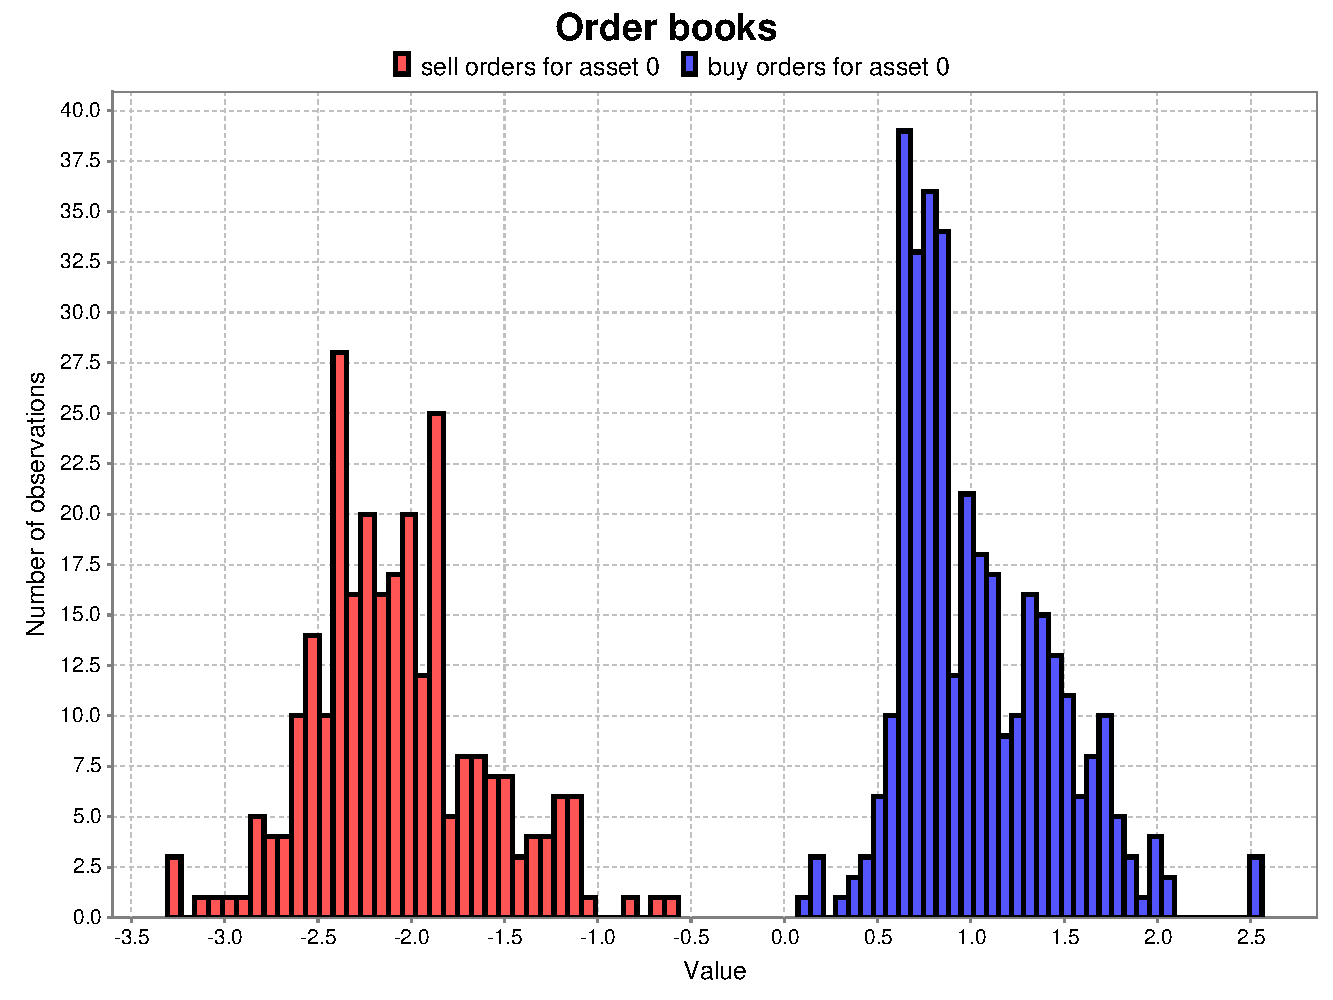
\includegraphics[width=1.00\textwidth]{../graphics/Farmer-orderbooks.pdf}}} 
      \quad
      \subfigure[Bid and ask log prices.]{\scalebox{0.5}{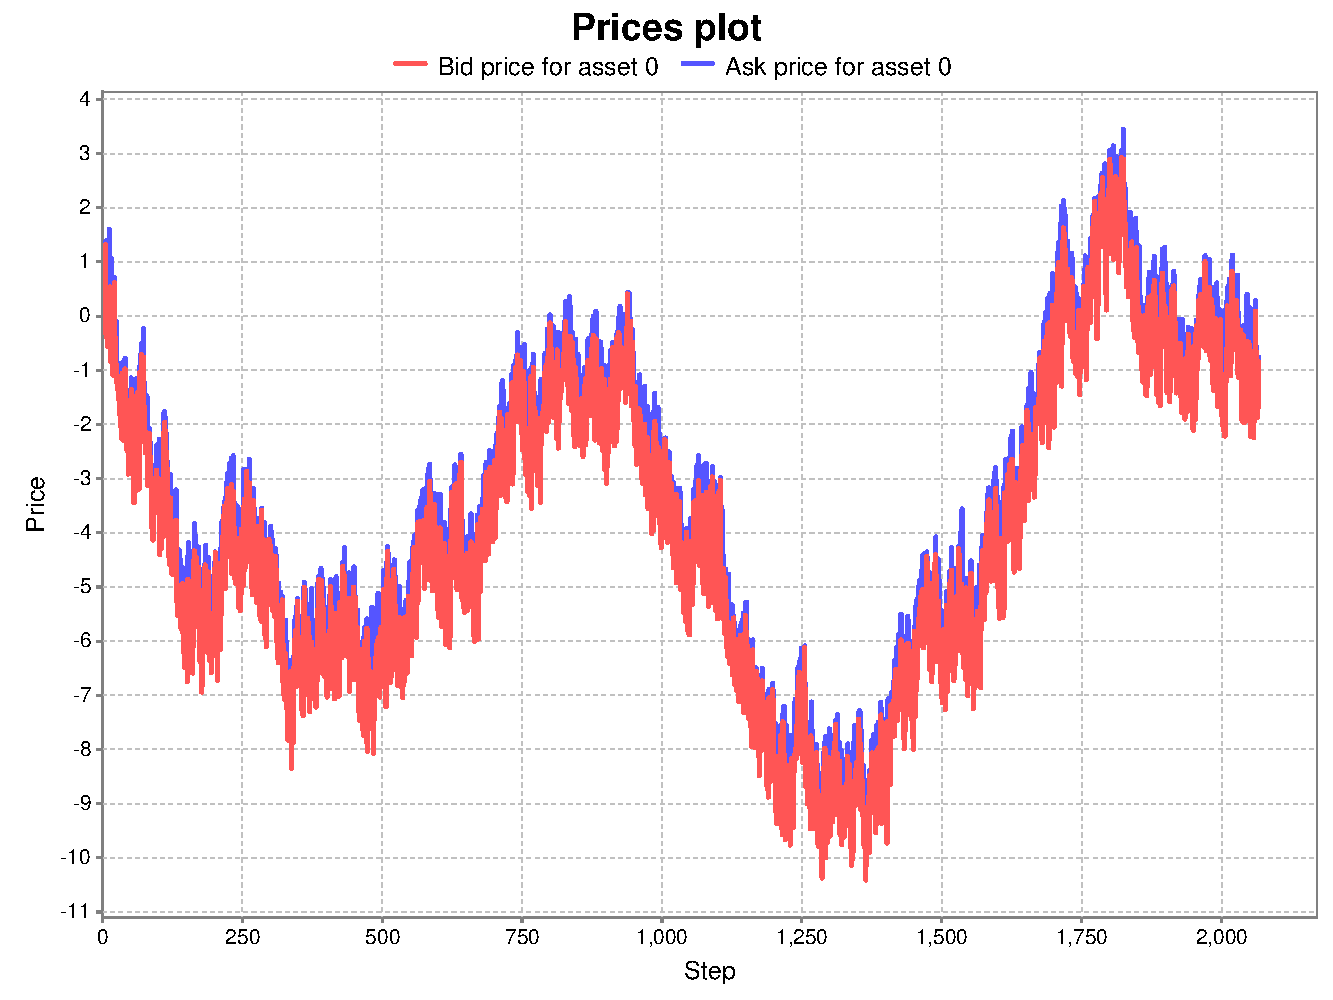
\includegraphics[width=1.00\textwidth]{../graphics/Farmer-pricesPlot.pdf}}}
}
   \mbox{
      \subfigure[Log returns histogram.]{\scalebox{0.5}{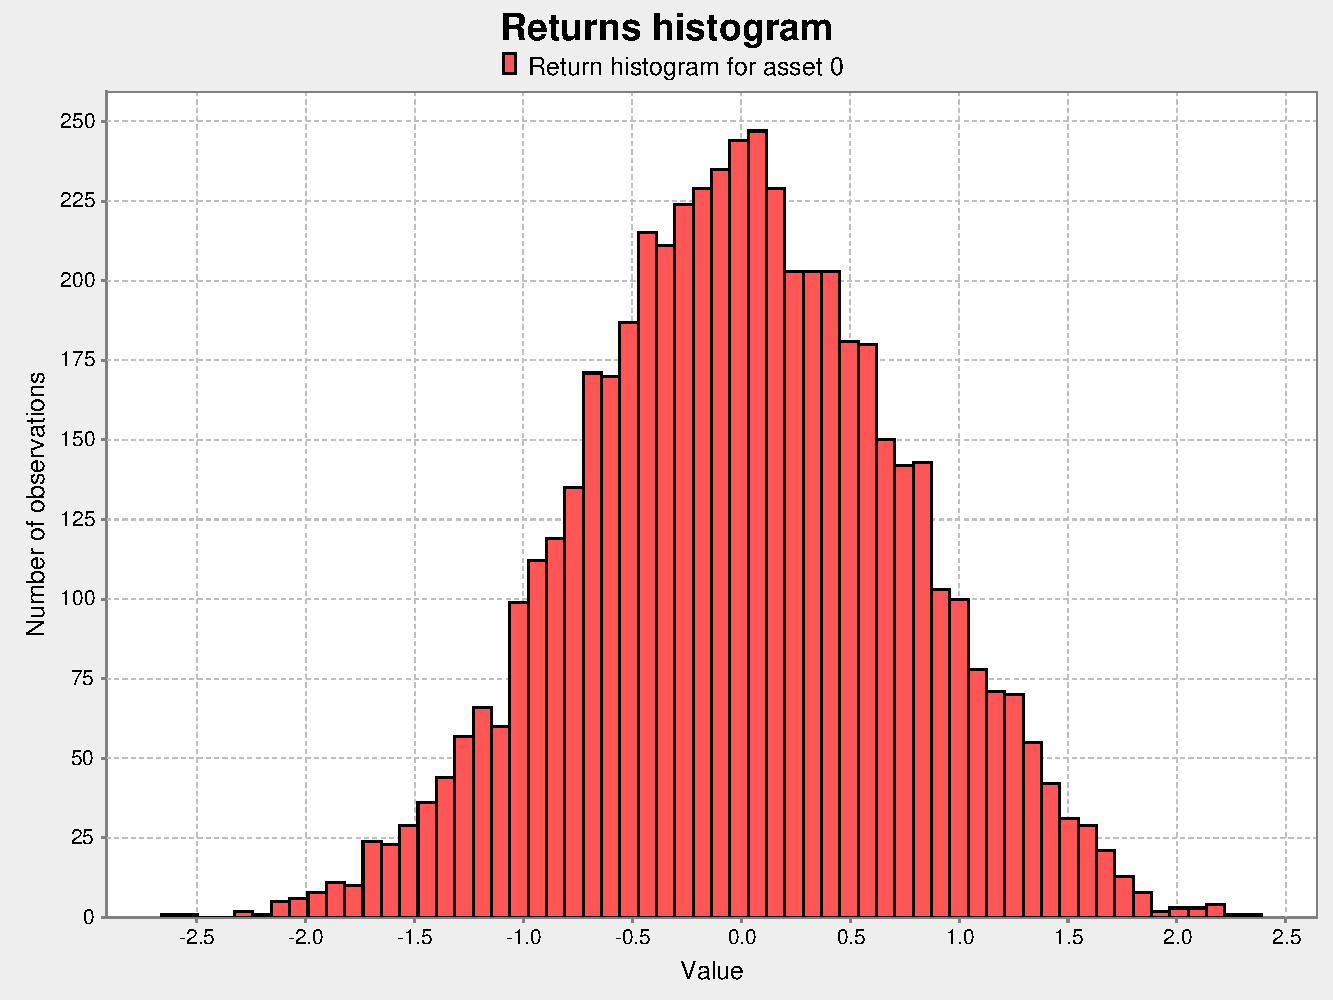
\includegraphics[width=1.00\textwidth]{../graphics/Farmer-returnsHistogram.pdf}}}
      \quad
      \subfigure[Trade volumes.]{\scalebox{0.5}{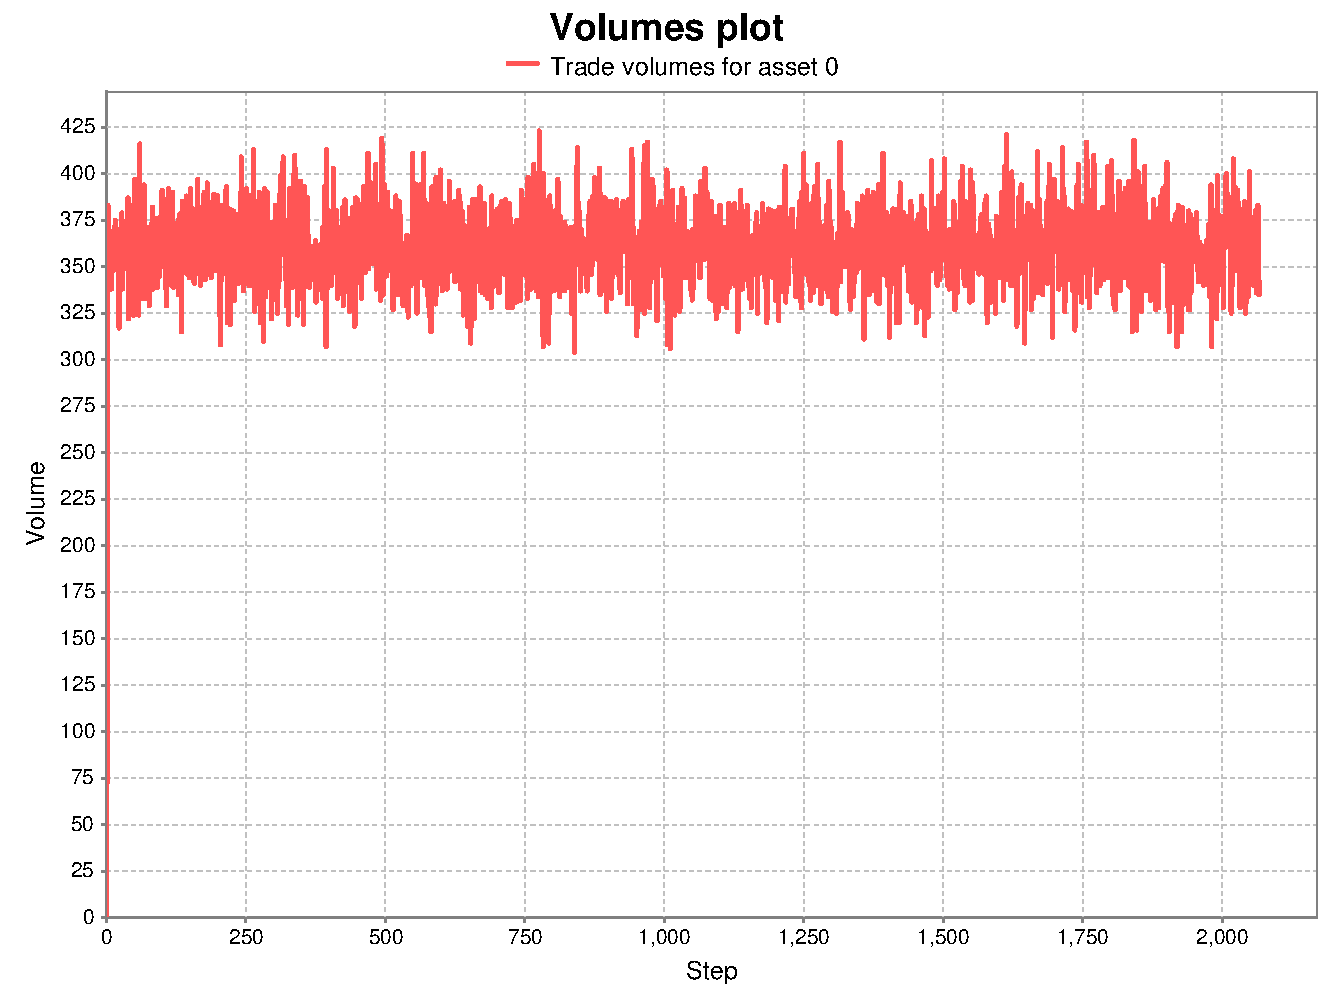
\includegraphics[width=1.00\textwidth]{../graphics/Farmer-volumesPlot.pdf}}}
      }
\mbox{
      \subfigure[Rolling Average Volatility.]{\scalebox{0.5}{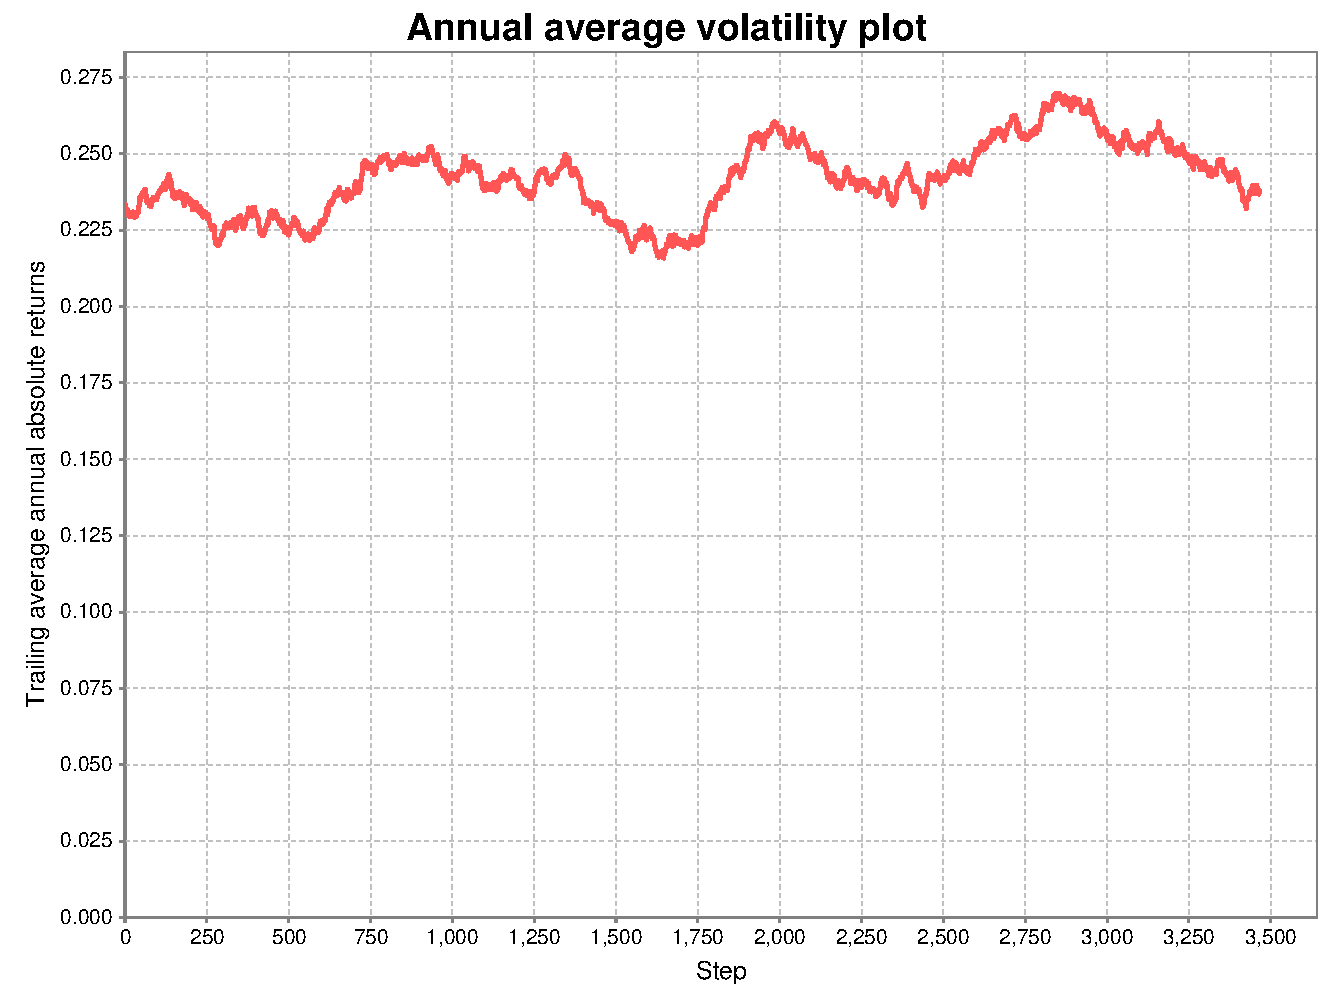
\includegraphics[width=1.0\textwidth]{../graphics/Farmer-avgVolatility.pdf}}}
      \quad
      \subfigure[Autocorrelation of returns.]{\scalebox{0.5}{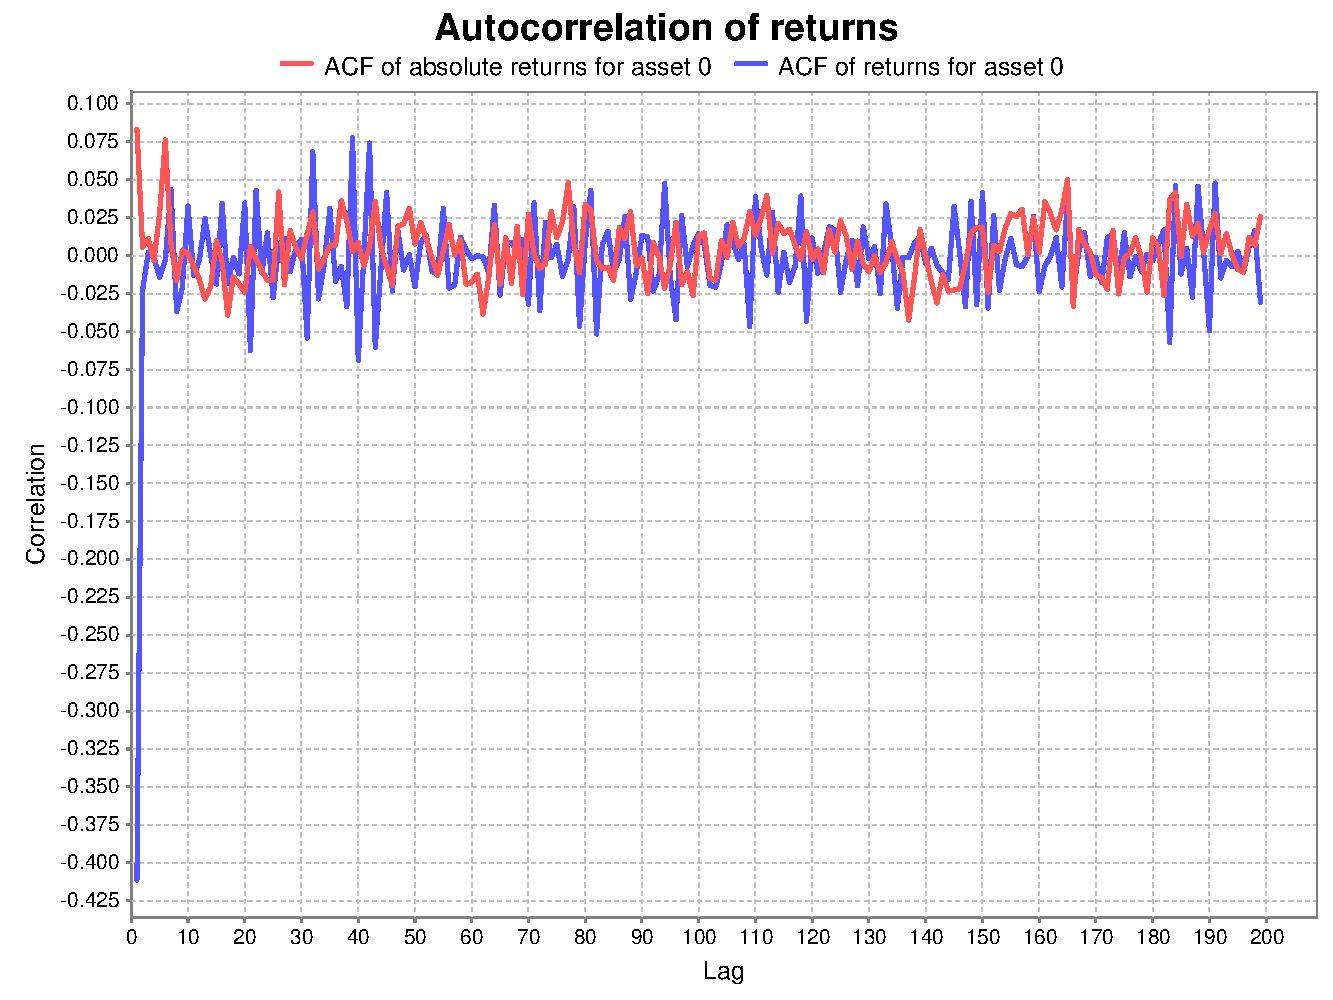
\includegraphics[width=1.00\textwidth]{../graphics/Farmer-acfReturns.pdf}}}
      }
\mbox{
      \subfigure[Raw and absolute log returns.]{\scalebox{0.6}{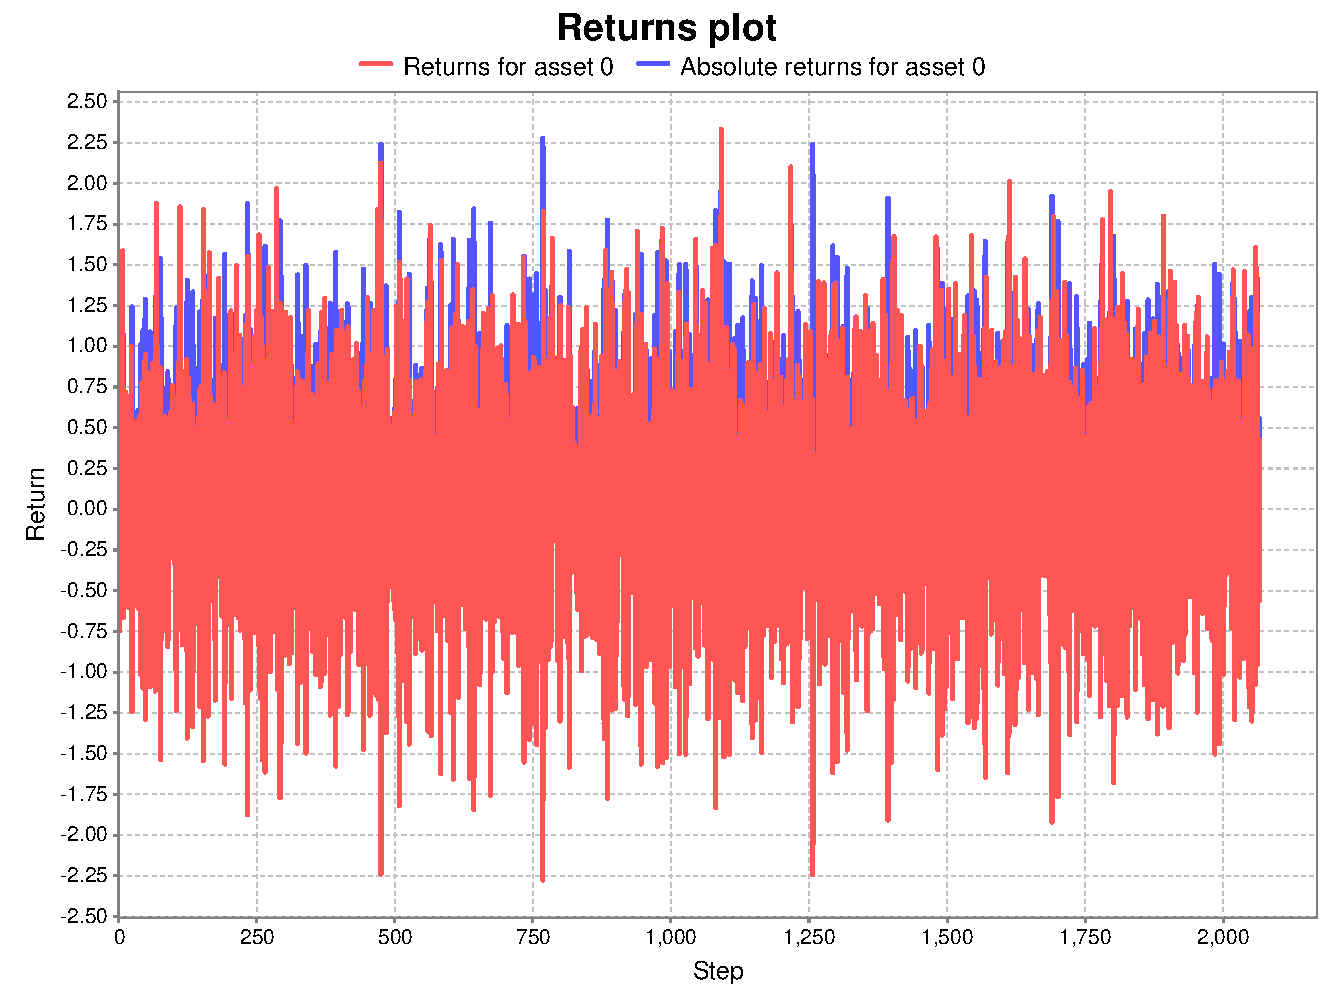
\includegraphics[width=1.00\textwidth]{../graphics/Farmer-returnPlot.pdf}}}
     }
    \caption{Examples of outputs and statistics from a single run of the Farmer FinancialModel simulation with $\alpha=.585$, $\delta=.39$, $\mu=.325$, $\sigma=1$. These parameters are derived from empirical data.}
    \label{fig:sampleDynamicsFarmer}
  \end{center}
\end{figure}

\begin{figure}[htbp]
  \begin{center}
   \mbox{
      \subfigure[Snapshot of Orderbook with actual prices (log x scale).]{\scalebox{0.6}{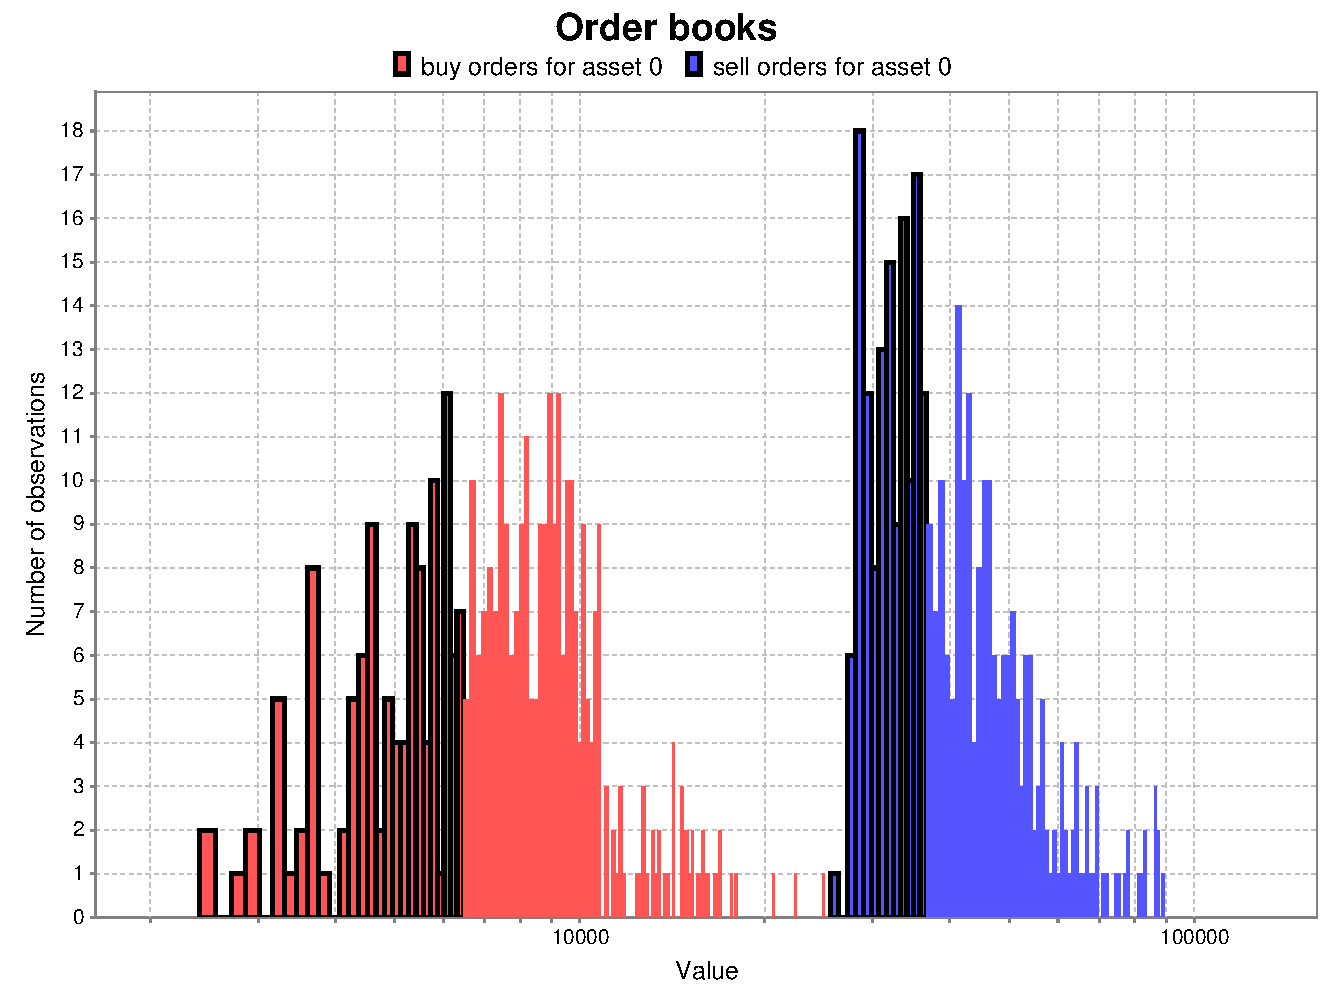
\includegraphics[width=1.00\textwidth]{../graphics/Farmer-linear-orderbooks.pdf}}} 
}
   \mbox{
\subfigure[Prices (log scale).]{\scalebox{0.5}{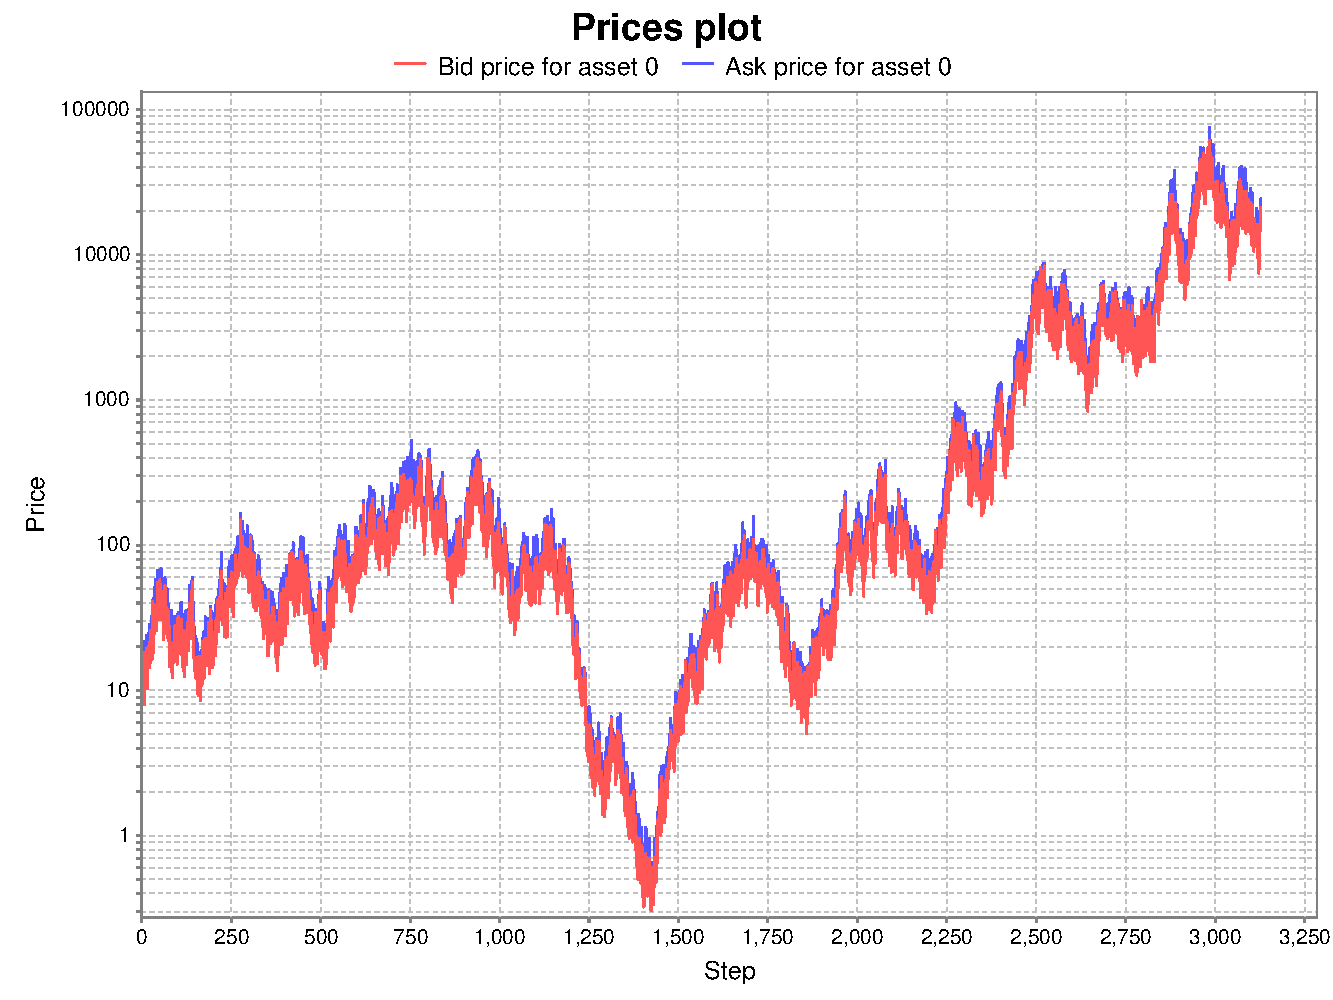
\includegraphics[width=1.00\textwidth]{../graphics/Farmer-linear-pricesPlot-logscale.pdf}}}
      \quad
\subfigure[Same prices (natural scale).]{\scalebox{0.5}{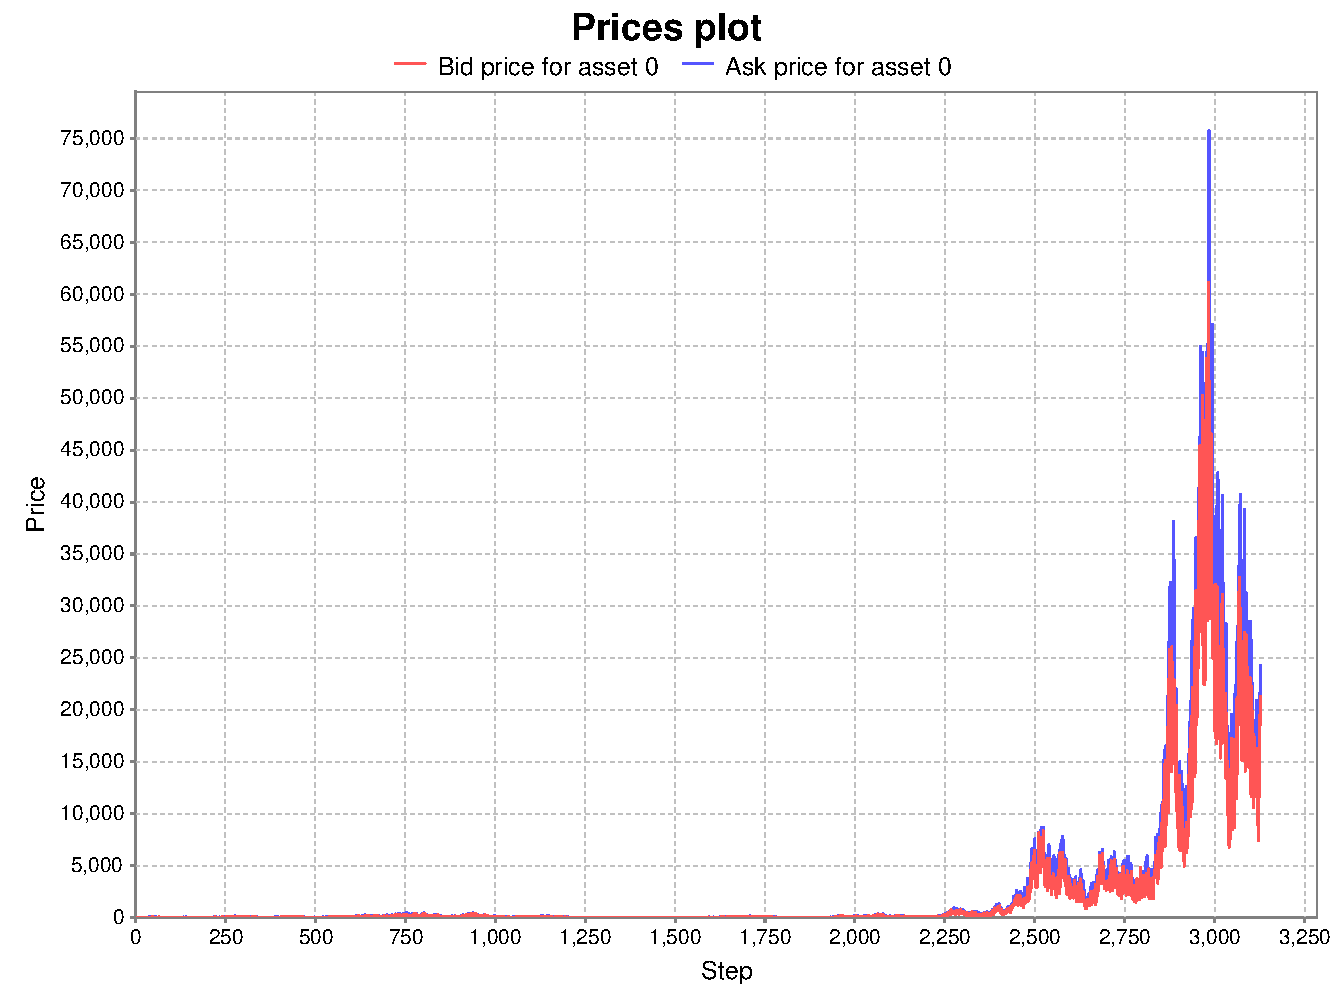
\includegraphics[width=1.00\textwidth]{../graphics/Farmer-linear-pricesPlot.pdf}}}
      }
    \caption{Examples of outputs and statistics from a single run of the FinancialModel simulation with $\alpha=.585$, $\delta=.39$, $\mu=.325$, $\sigma=1$. These parameters are derived from empirical data.}
    \label{fig:dynamicsFarmerNonLog}
  \end{center}
\end{figure}


\subsection{Farmer-Cont Model}

As an experiment, we constructed a model combining some aspects of the Farmer model with some aspects of the Cont model. The result is a model which is still essentially zero intelligence, but which exhibits empirically positive characteristics of both models. In this model there are two types of agents, which interact via the continuous double auction mechanism, as in Farmer. In fact, the Patient traders, which place limit orders and thus provide liquidity, remain the same. Impatient traders are modeled after Cont. They have heterogeneous volatility thresholds, and place market orders depending upon how public information in the form of a normally distributed random variable $\epsilon_t ~ N(0,D^2)$ compares with these thresholds. Some fraction $s$ of agents then adjust their volatility thresholds in light of current volatility by setting it to the trailing period's return rate.

\paragraph*{}
The result is shown in Figure \ref{fig:FarmerContDynamics}. When there are sufficient limit orders being placed by Farmer's patient agents to ensure adequate liquidity for Market orders, we get dynamics that have many positive aspects compared with reality --- approximately power law return distribution, volatility clustering, realistic variability in linear prices, volumes, and returns, and essentially no predictability of future returns based upon past returns.

\begin{figure}[htbp]
  \begin{center}
   \mbox{
      \subfigure[Trade volumes.]{\scalebox{0.33}{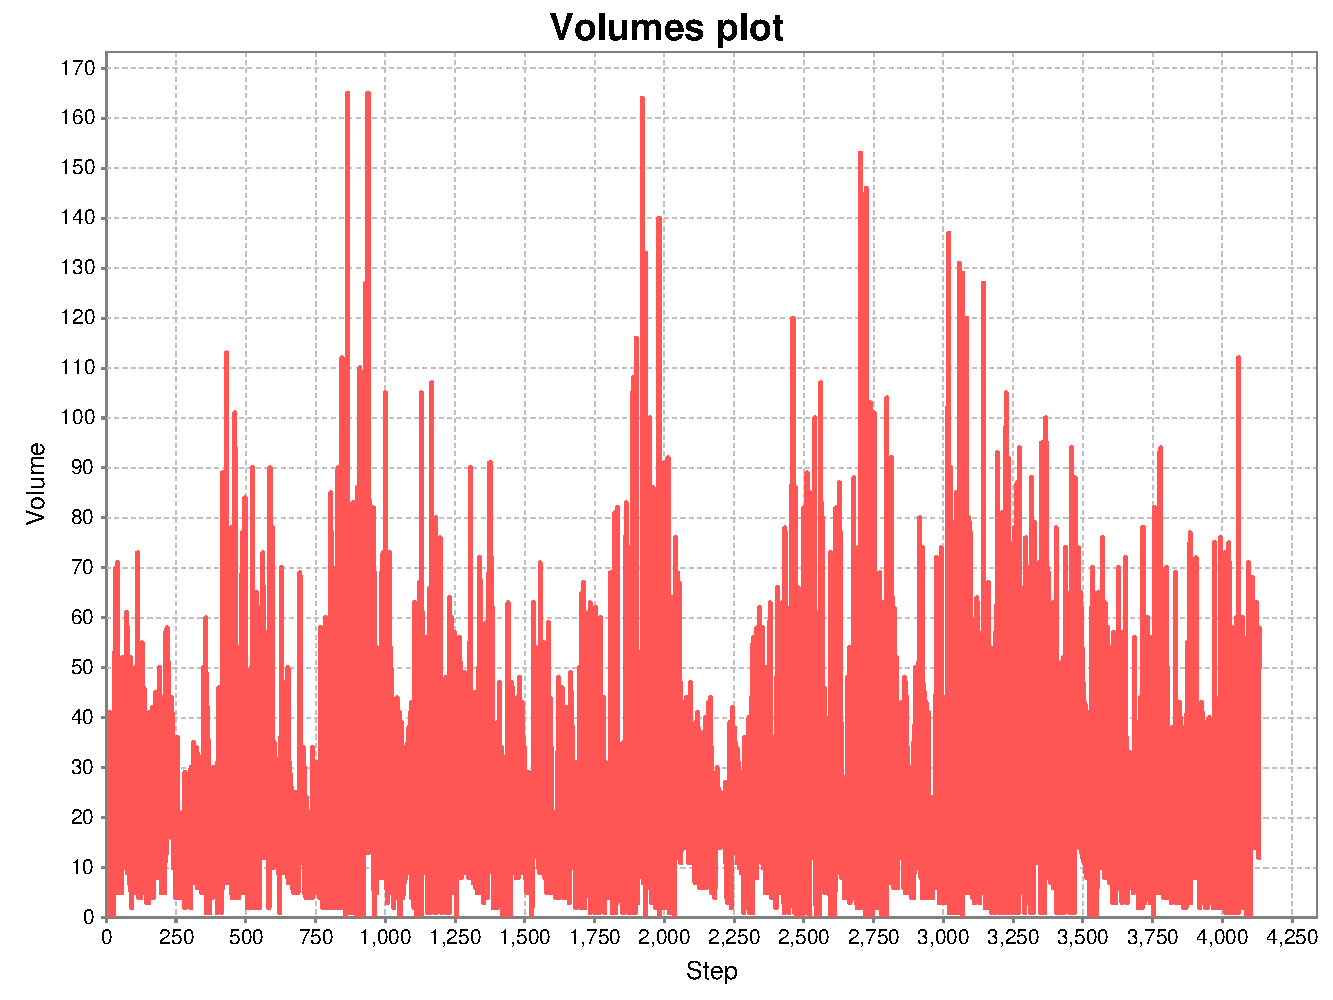
\includegraphics[width=1.00\textwidth]{../graphics/FC-volumesPlot.pdf}}}
      \quad
      \subfigure[Price]{\scalebox{0.33}{ 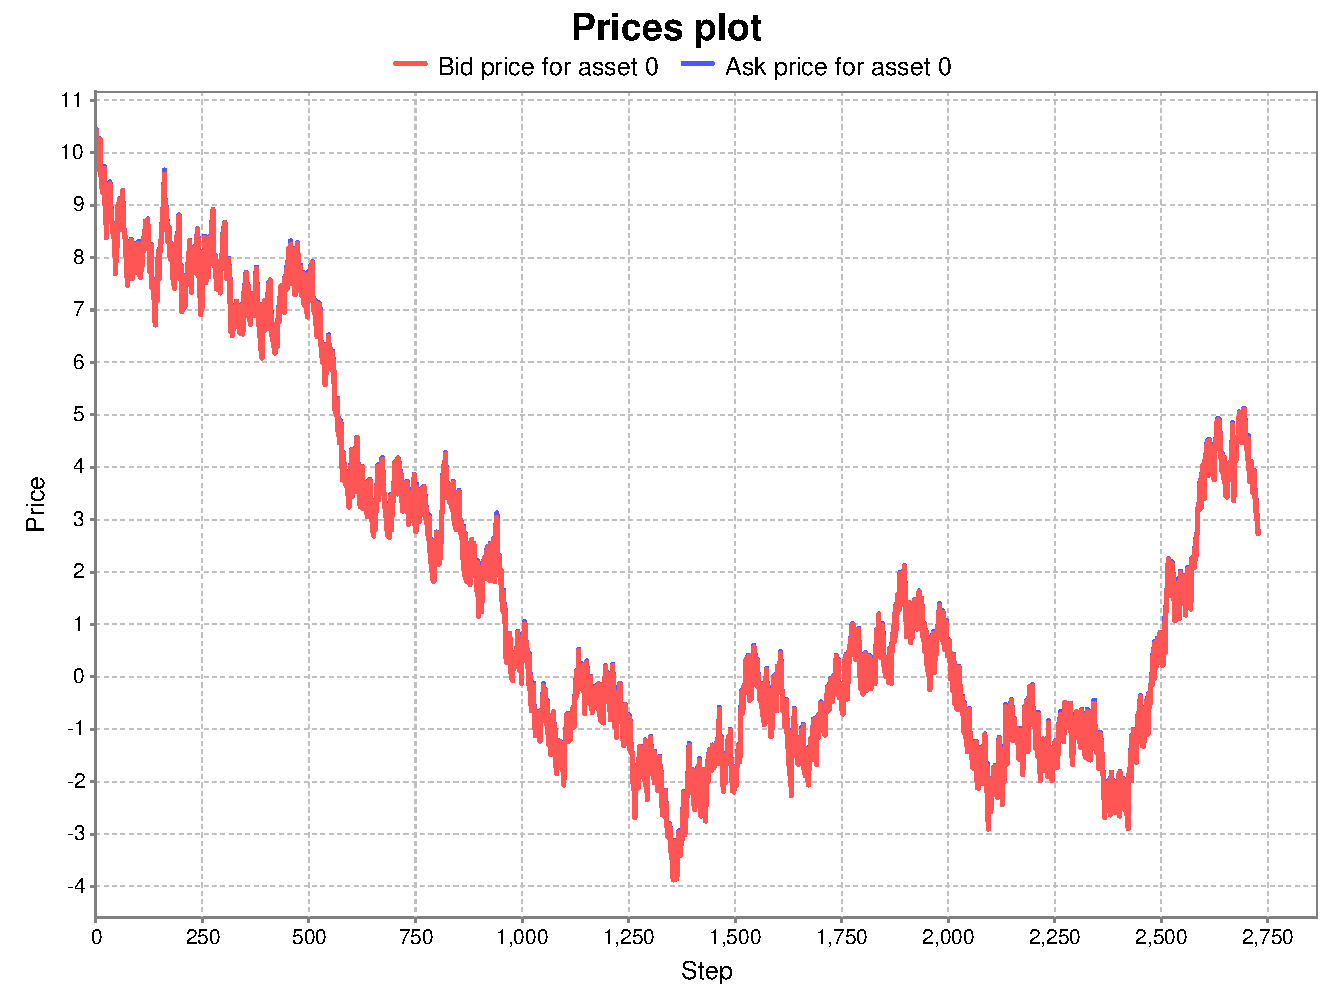
\includegraphics[width=1.0\textwidth]{../graphics/FC-pricesPlot.pdf}}} \quad
      }
    \mbox{
      \subfigure[Raw and absolute log returns.]{\scalebox{0.33}{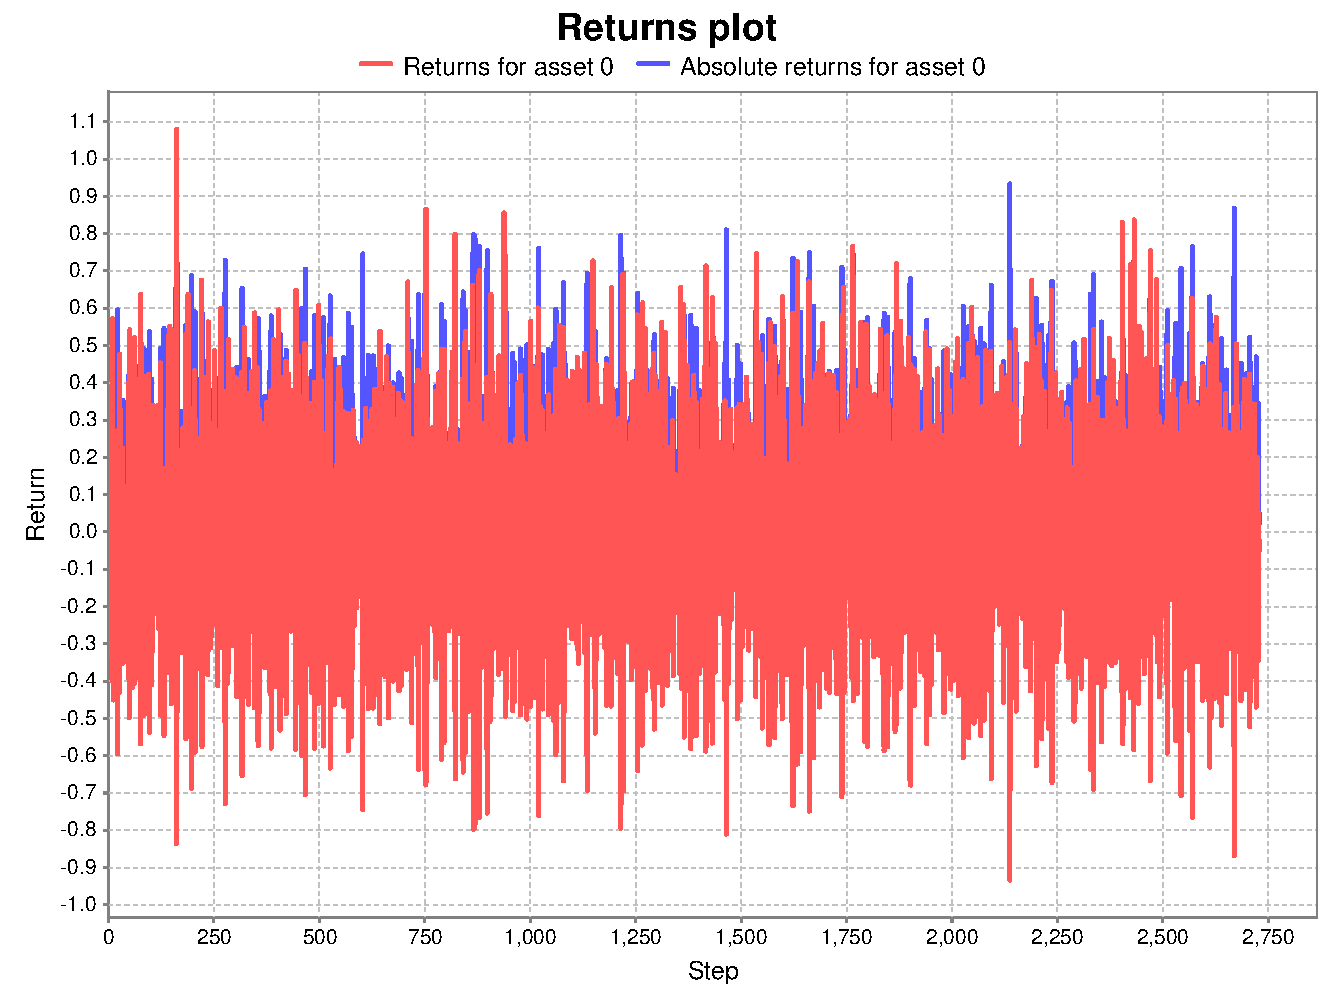
\includegraphics[width=1.00\textwidth]{../graphics/FC-returnsPlot.pdf}}}
      \quad
      \subfigure[Returns histogram.]{\scalebox{0.33}{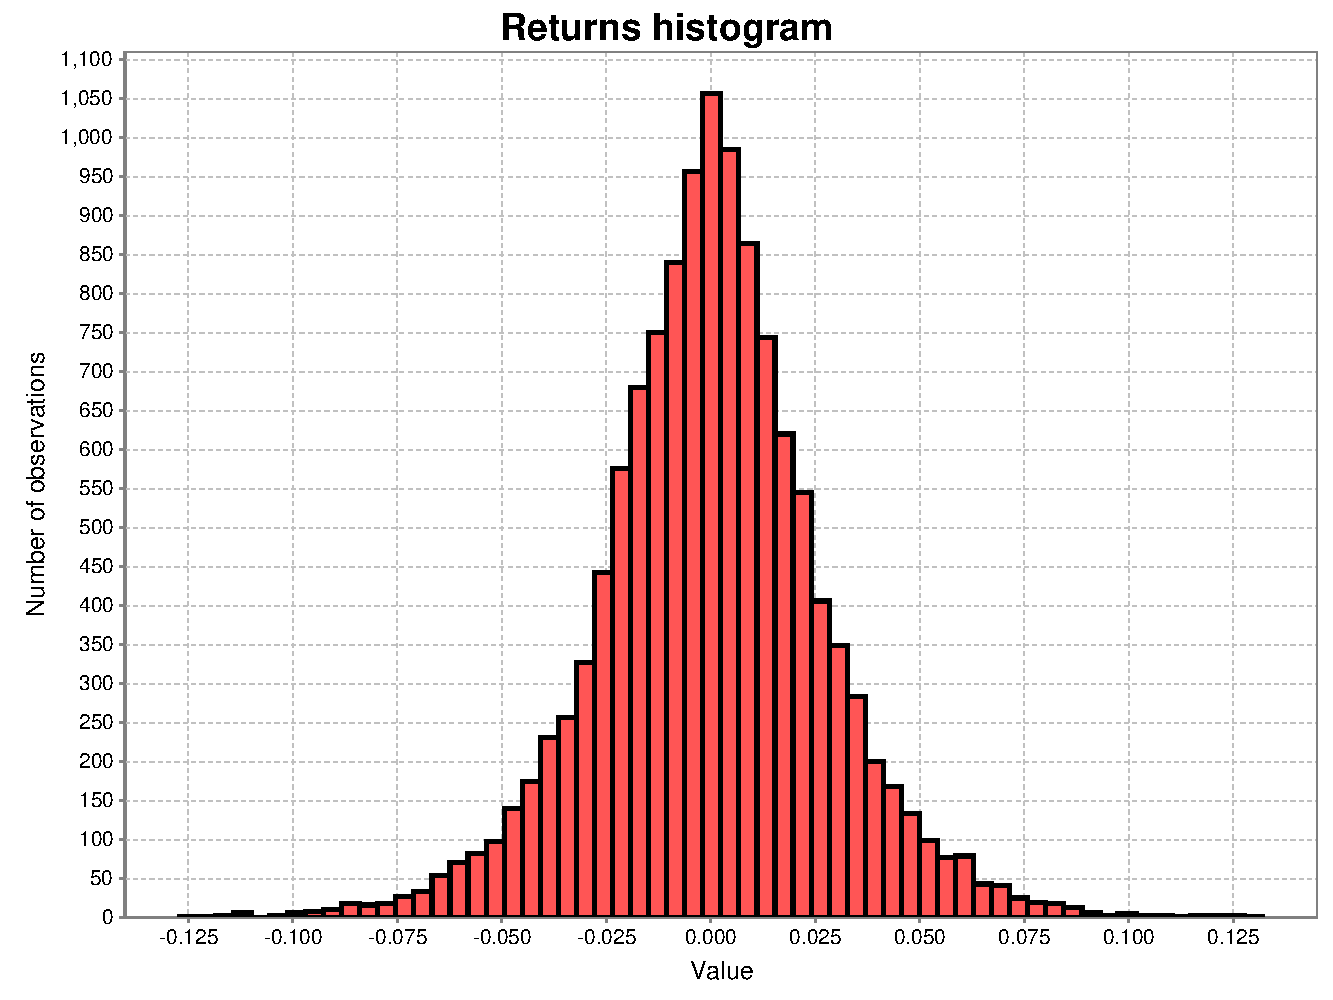
\includegraphics[width=1.00\textwidth]{../graphics/FC-returnsHistogram.pdf}}}
      \quad
      \subfigure[Returns histogram in logs.]{\scalebox{0.33}{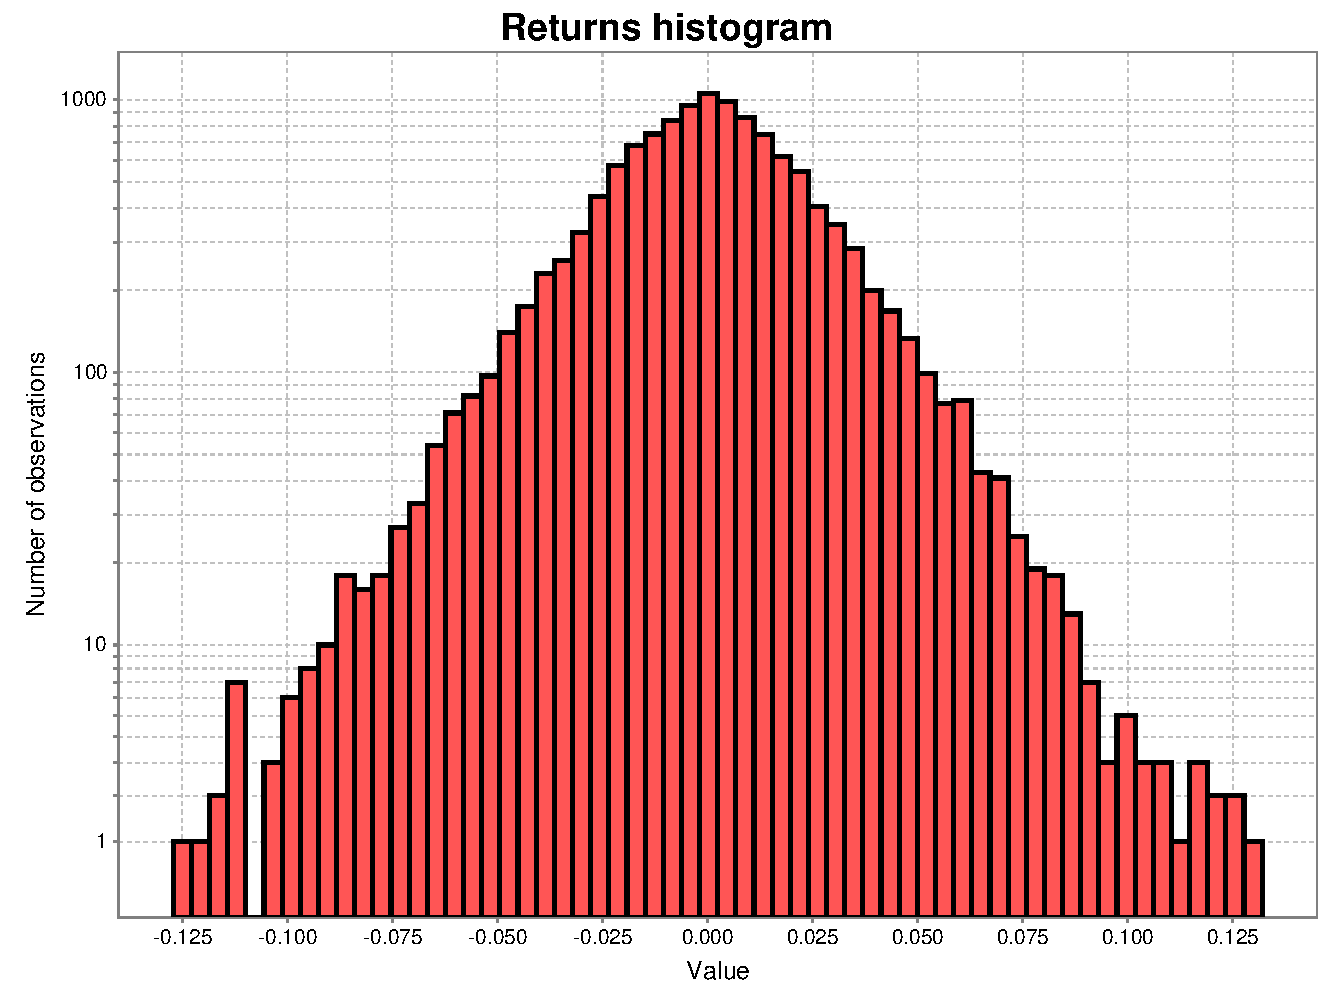
\includegraphics[width=1.00\textwidth]{../graphics/FC-logReturnsHistogram.pdf}}}       
}
    \mbox{
      \subfigure[Annualized moving average volatility]{\scalebox{0.33}{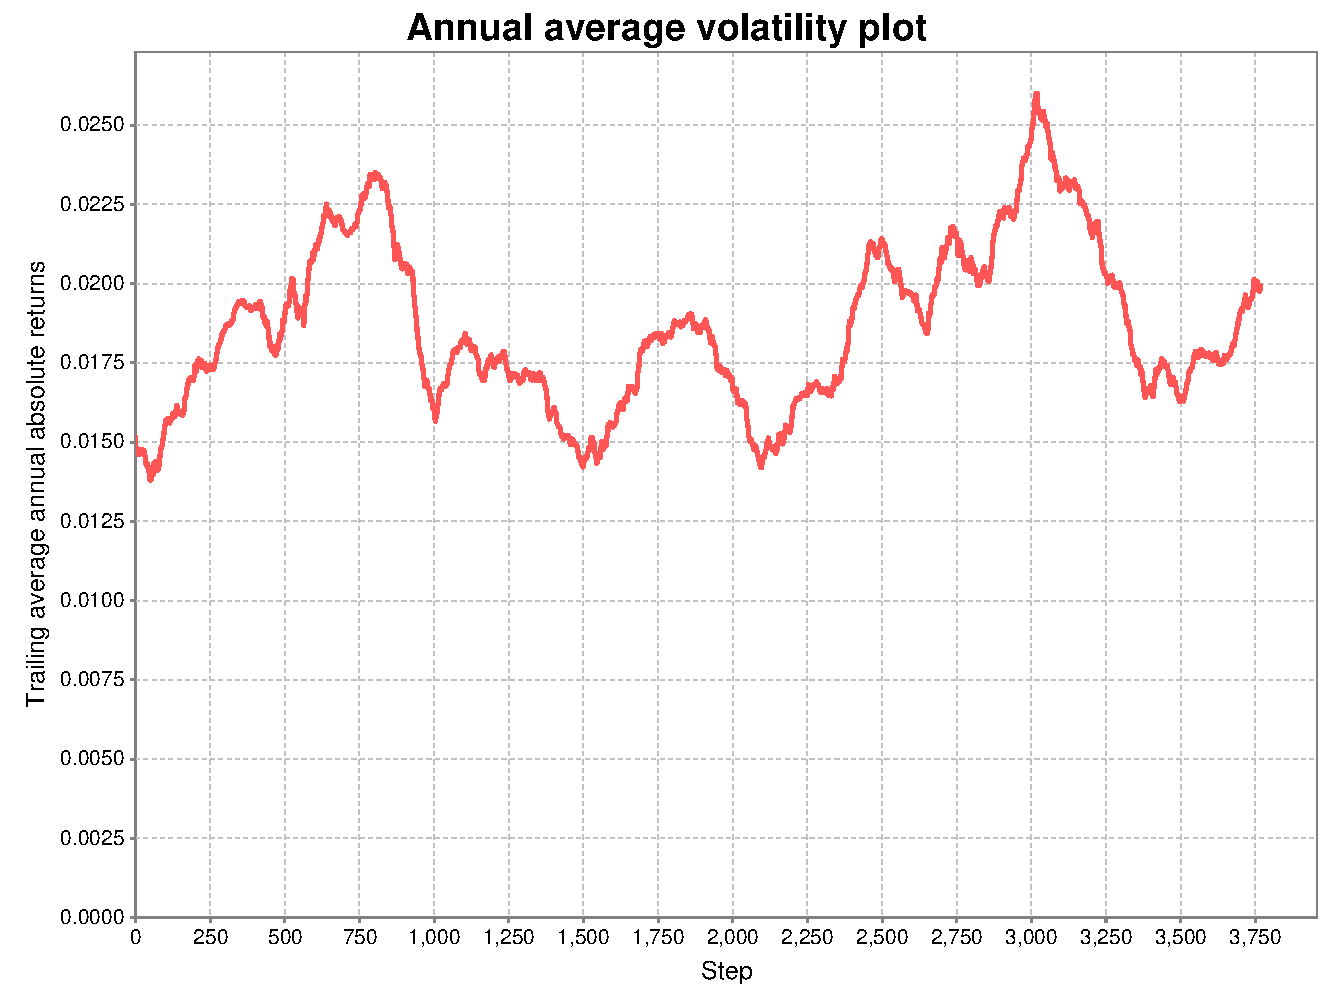
\includegraphics[width=1.00\textwidth]{../graphics/FC-avgVolatility.pdf}}}
      \quad
      \subfigure[Snapshot of orderbook.]{\scalebox{0.33}{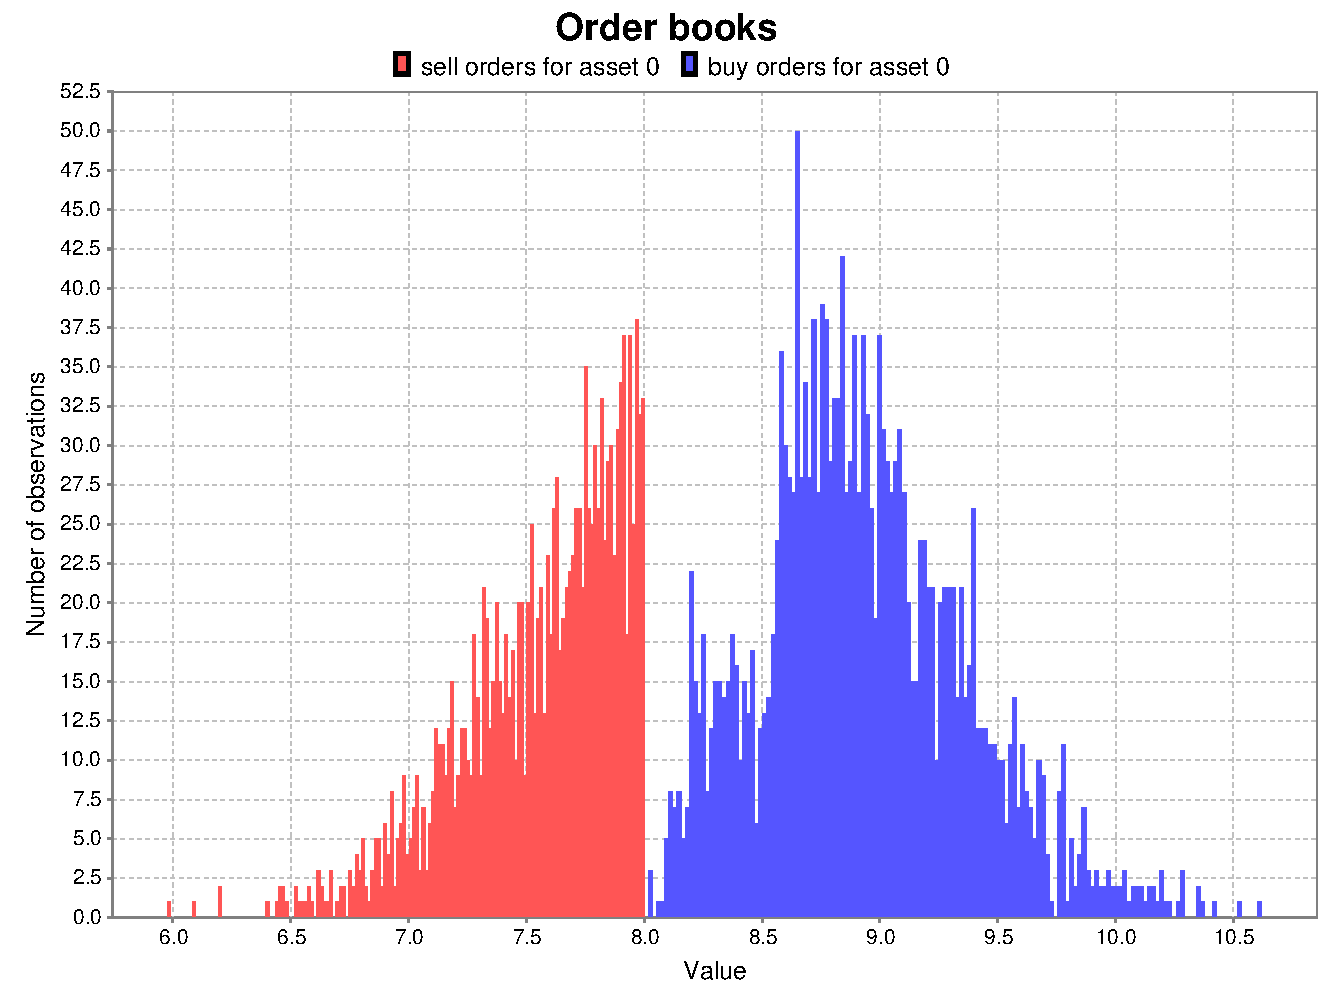
\includegraphics[width=1.00\textwidth]{../graphics/FC-orderbooks.pdf}}}
      \quad
      \subfigure[Autocorrelation of returns.]{\scalebox{0.33}{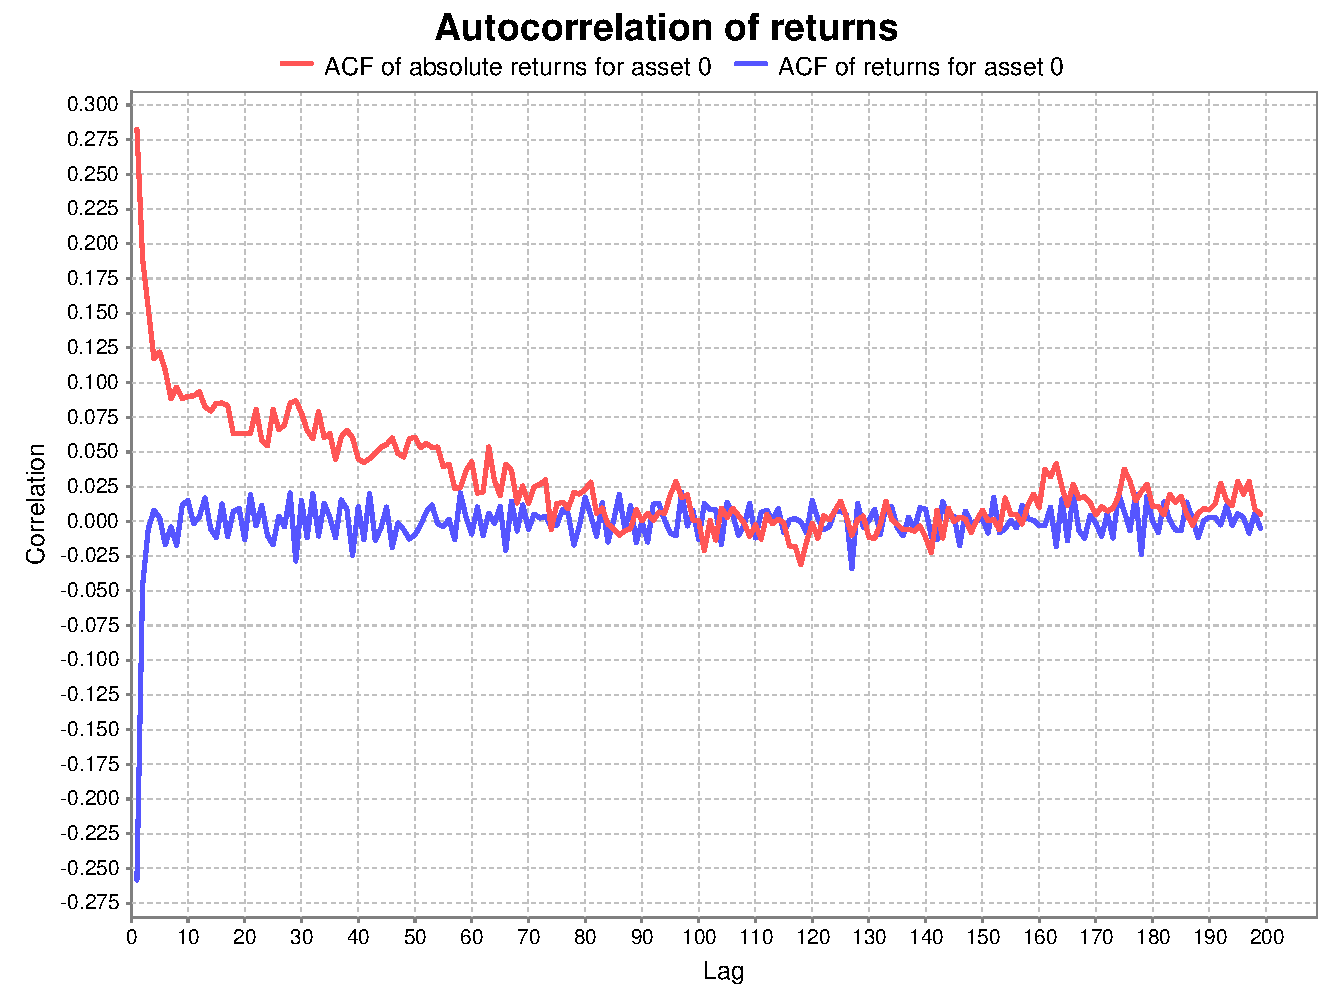
\includegraphics[width=1.00\textwidth]{../graphics/FC-acfReturns.pdf}}}
      }
    \caption{Examples of outputs and statistics from a single run of the Farmer-Cont hybrid FinancialModel simulation with actual prices, $D=0.001$, $s=0.01$, $\alpha=0.9$, $\delta=0.2$, and $\mu=0.4$.}
    \label{fig:FarmerContDynamics}
  \end{center}
\end{figure}

\subsection{Westerhoff Model}

The Westerhoff model (\cite{westerhoff2004}) includes a limited number of markets in which two types of agents operate. Fundamentalists specialize in a certain market while chartists may switch between markets. More specifically, chartists use extrapolative methods to select markets that shows price trends but that are not too misaligned.

The model considers $k = 1,2\dots K$ asset markets of equal size: the log fundamental value of asset $k$ in period $t + 1$ is regulated by a news arrival process:
\begin{equation*}
F_{t+1}^k = F_t^k + N
\end{equation*}

Market makers are present in all markets and stand ready to absorb imbalances between buyers and sellers: they adjust prices $S^k_t$ according to a loglinear price impact function.
Traders submit orders according to their expectations of the price movements. Fundamentalist expect the prices of the assets to return to their fundamental values and their demand is expressed as:
\begin{align*}
D_t^{F,k} &= a^F[E_t^F(S^k_{t+1}) - S^k_{t}],\\
E_t^F &= S^k_{t} + b^F(F_t^k - S^k_t)
\end{align*}
On the other hand, chartists follow simple technical analysis rules:
\begin{align*}
D_t^{C,k} &= a^C[E_t^C(S^k_{t+1}) - S^k_{t}],\\
E_t^C &= S^k_{t} + b^C(S_t^k - S^k_{t-1})
\end{align*}

Chartists try to identify the attractiveness of markets with a fitness measure that entails the risk of being captured in a bursting bubble. The attractiveness of market $k$ is defined as:
\begin{equation*}
A^k_t = \log \frac{1}{1+f(F_t^k - S^k_t)^2}
\end{equation*}
The relative percentage of chartists choosing market $k$ depends on the attractiveness of that market and is defined as:
\begin{equation*}
W^k_t = \frac{\exp(gA^k_t)}{\sum_{k=1}^K \exp(gA^k_t)}
\end{equation*}
As shown in Figure \ref{fig:Westerhoffsim}, this model is capable of  generating complex price dynamics, volatility clustering, fat tails for the distribution of the returns and positive autocorrelation for absolute returns.
\begin{figure}[htbp]
  \begin{center}
   \mbox{
      \subfigure[Log price $S^1$]{\scalebox{0.33}{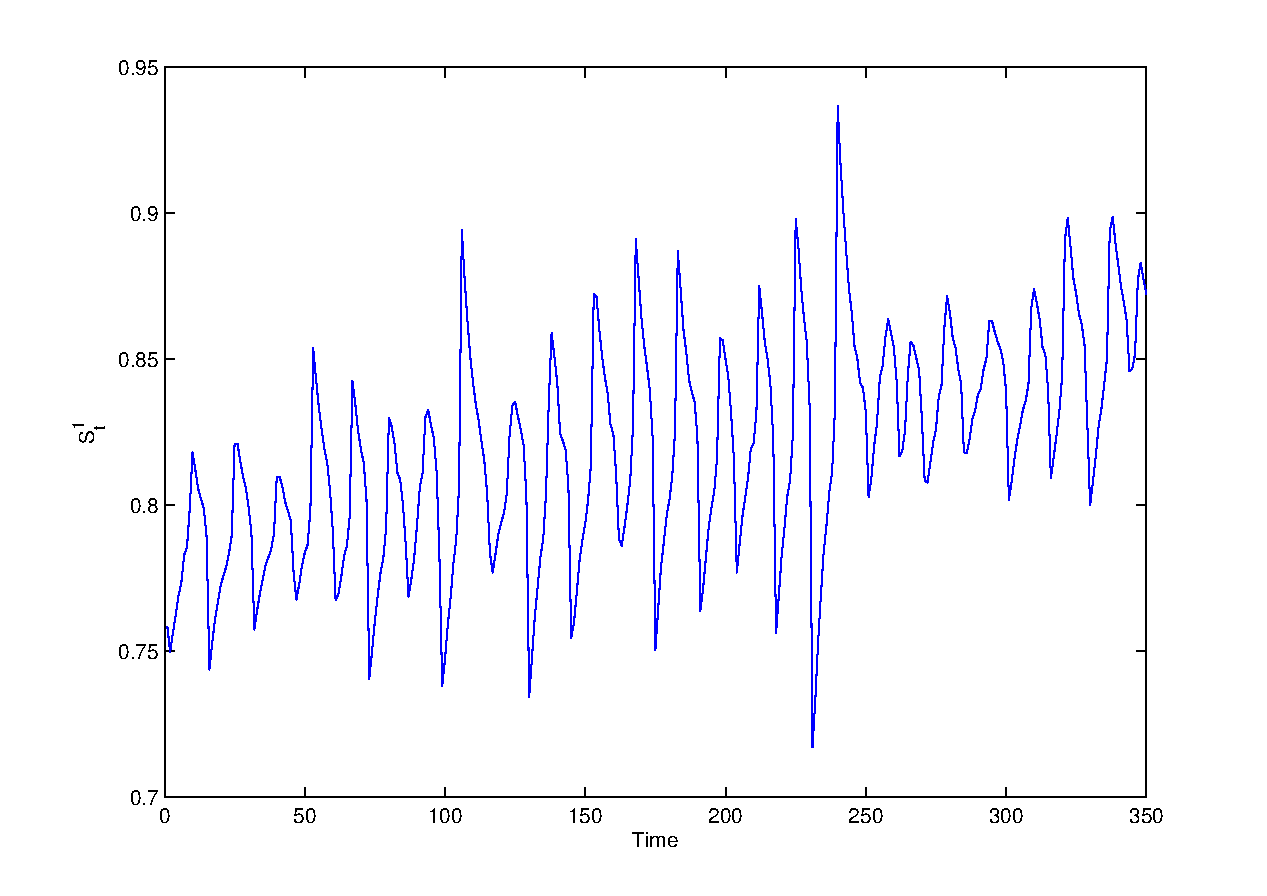
\includegraphics[width=1.00\textwidth]{../graphics/s1dyn.pdf}}}
      \quad
      \subfigure[Log price index]{\scalebox{0.33}{ 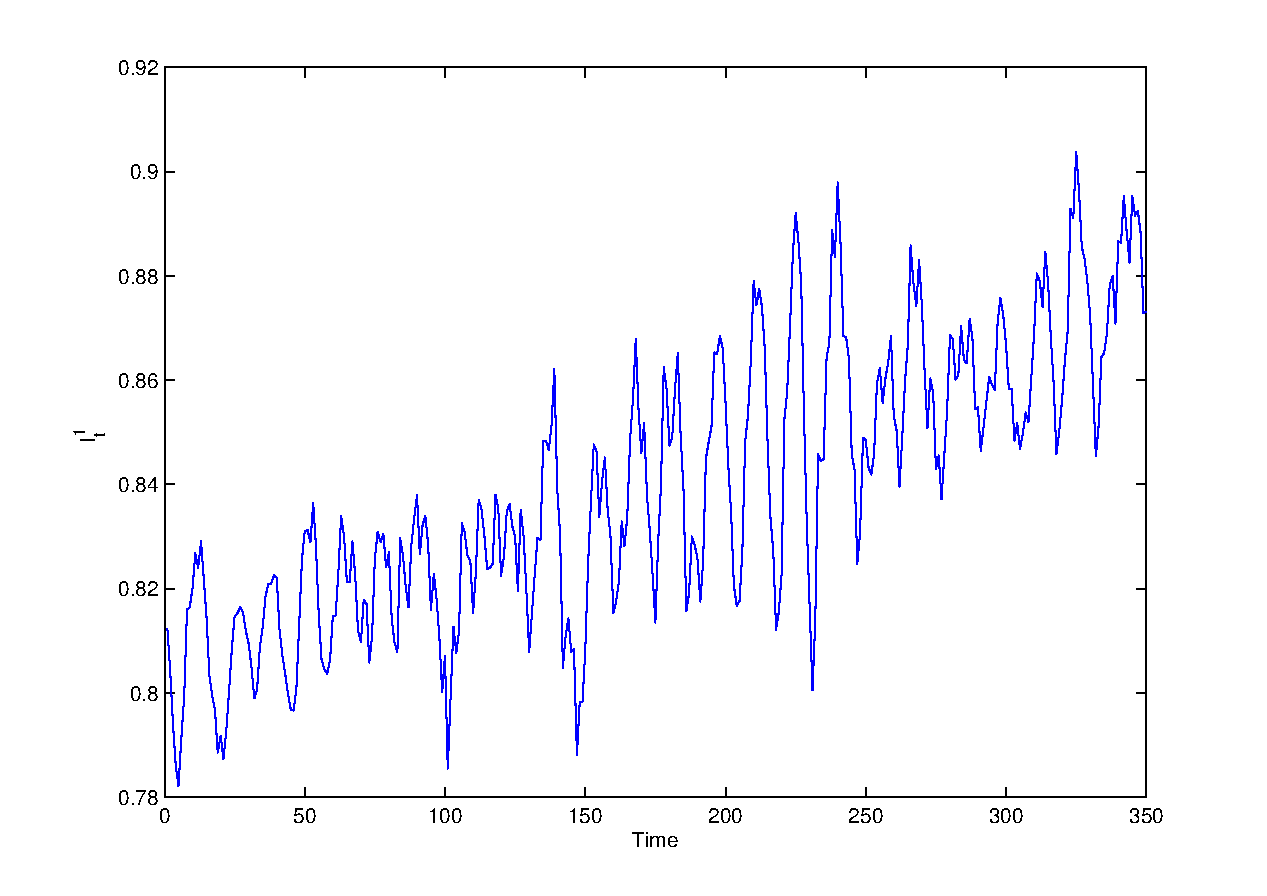
\includegraphics[width=1.0\textwidth]{../graphics/Idyn.pdf}}} \quad
      \subfigure[Fraction of chartist in market 1]{\scalebox{0.33}{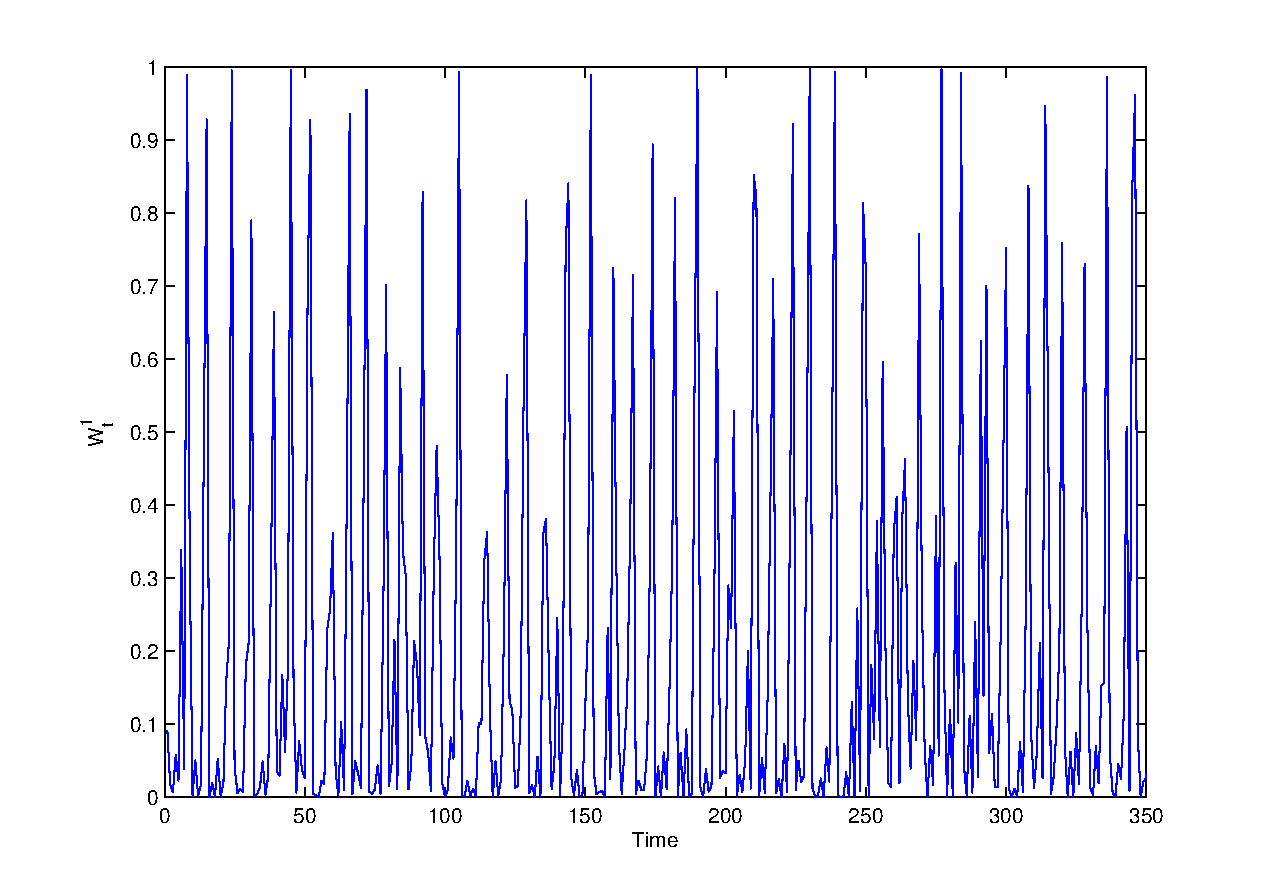
\includegraphics[width=1.00\textwidth]{../graphics/w1dyn.pdf}}}
      }
    \mbox{
      \subfigure[Raw returns of asset 1]{\scalebox{0.33}{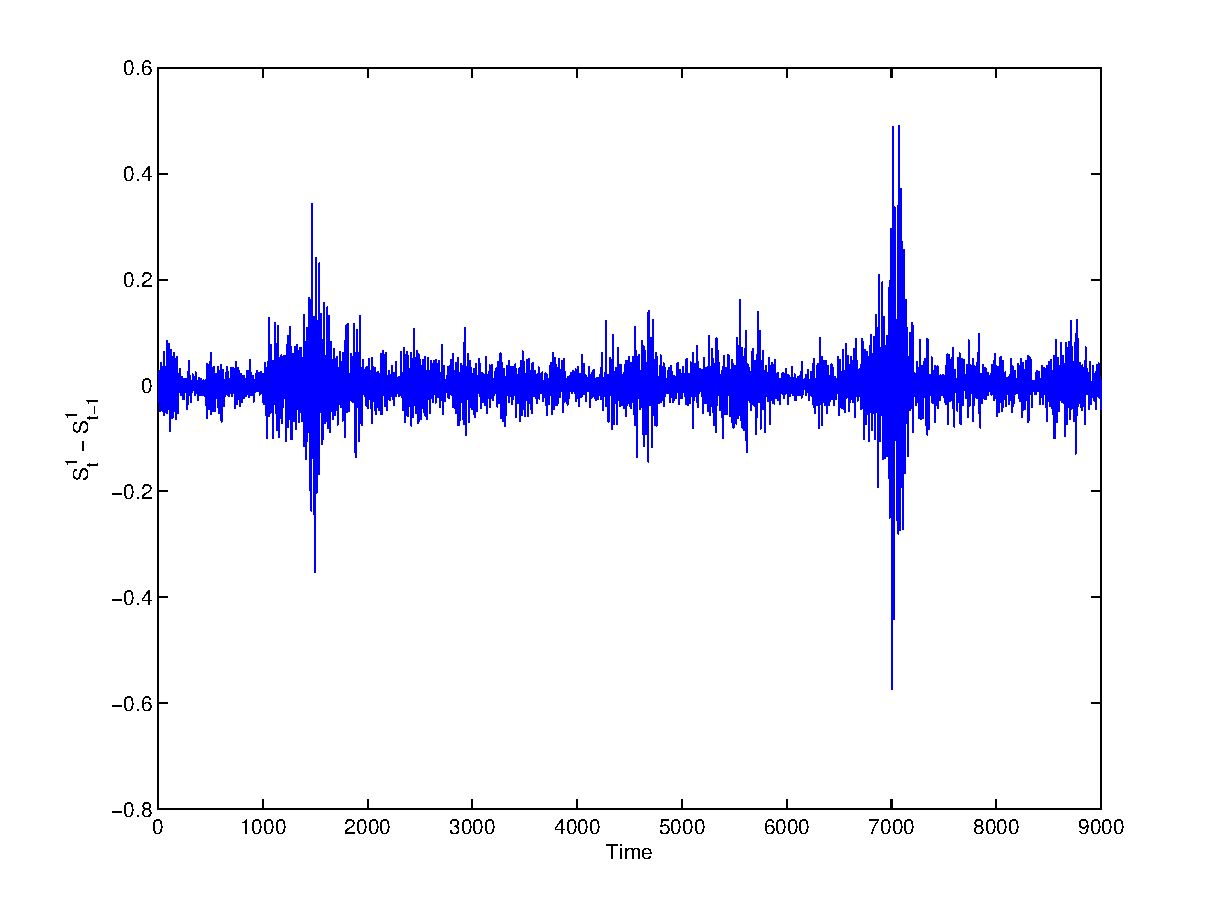
\includegraphics[width=1.00\textwidth]{../graphics/rets1.pdf}}}
      \quad
      \subfigure[Raw returns of price index ]{\scalebox{0.33}{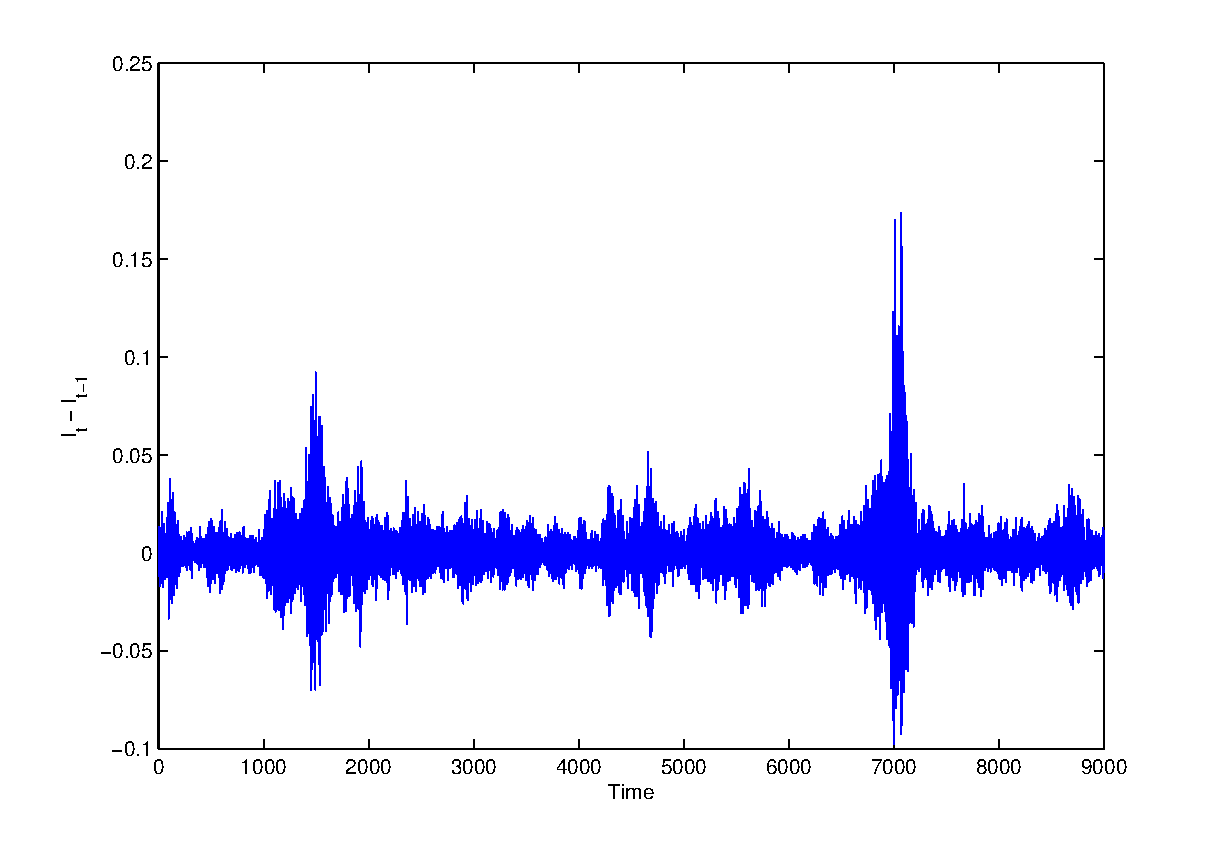
\includegraphics[width=1.00\textwidth]{../graphics/retI.pdf}}}
      \quad
       \subfigure[Attractor for log price changes of asset 1]{\scalebox{0.33}{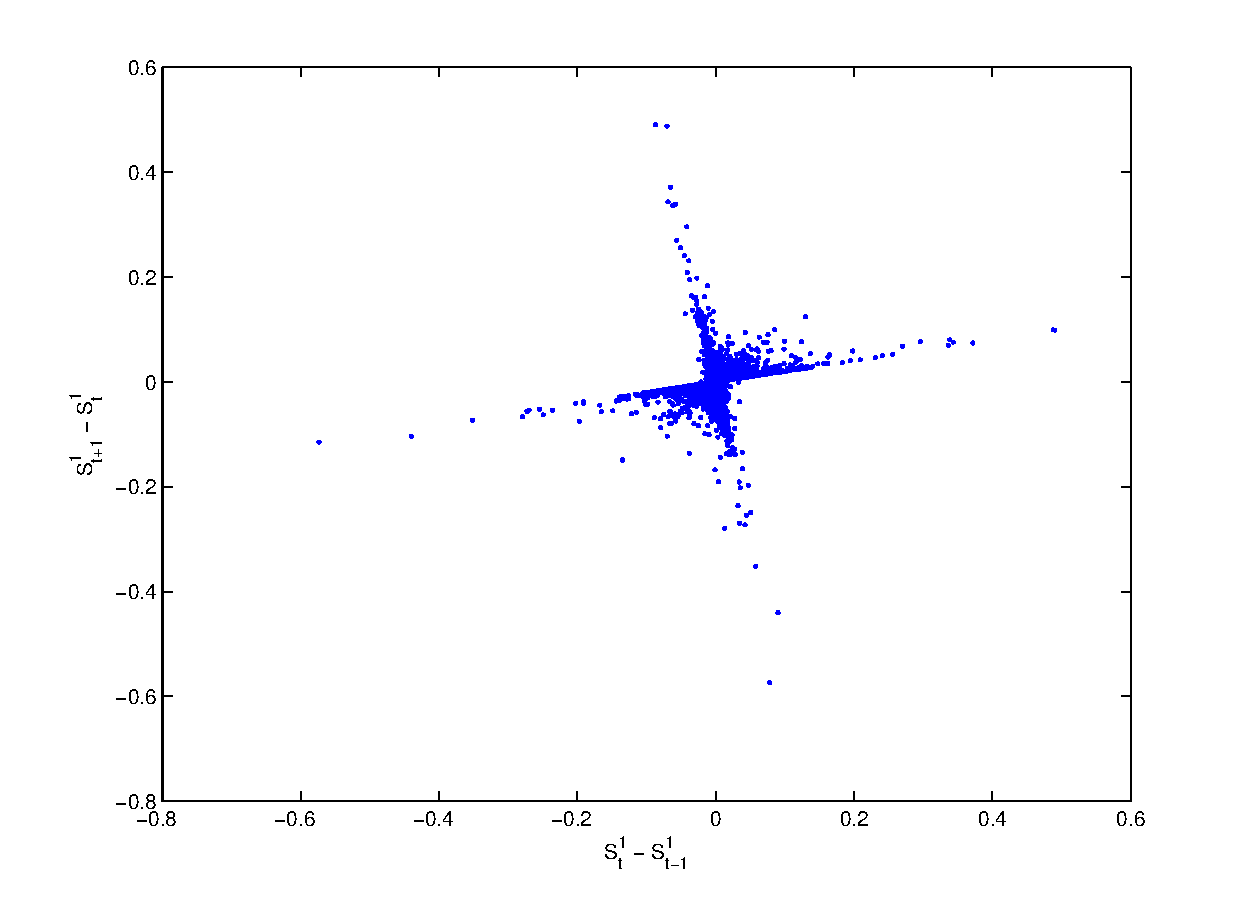
\includegraphics[width=1.00\textwidth]{../graphics/phasespaceS1.pdf}}}   
   }
    \mbox{
      \subfigure[Attractor for price index changes]{\scalebox{0.33}{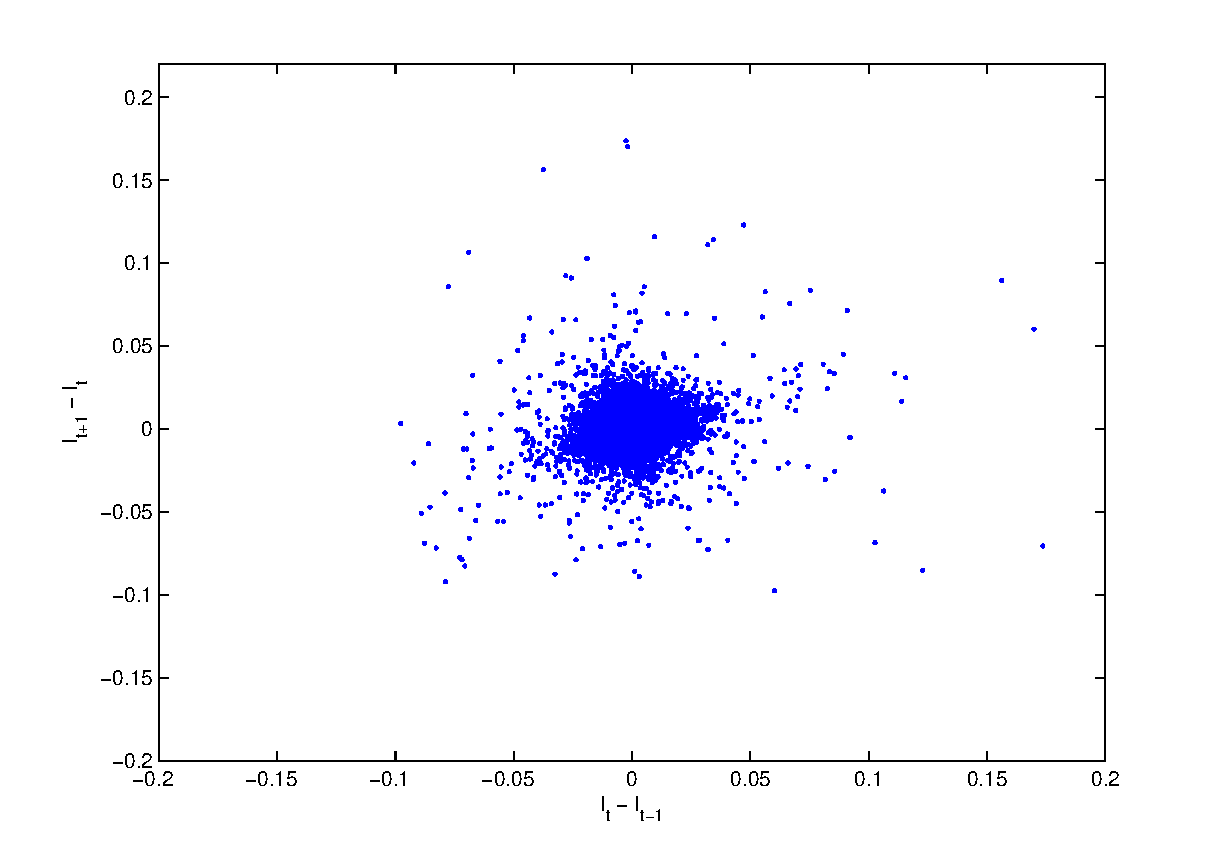
\includegraphics[width=1.00\textwidth]{../graphics/phasespaceI.pdf}}}
      \quad
      \subfigure[Autocorrelation for raw returns of asset 1]{\scalebox{0.33}{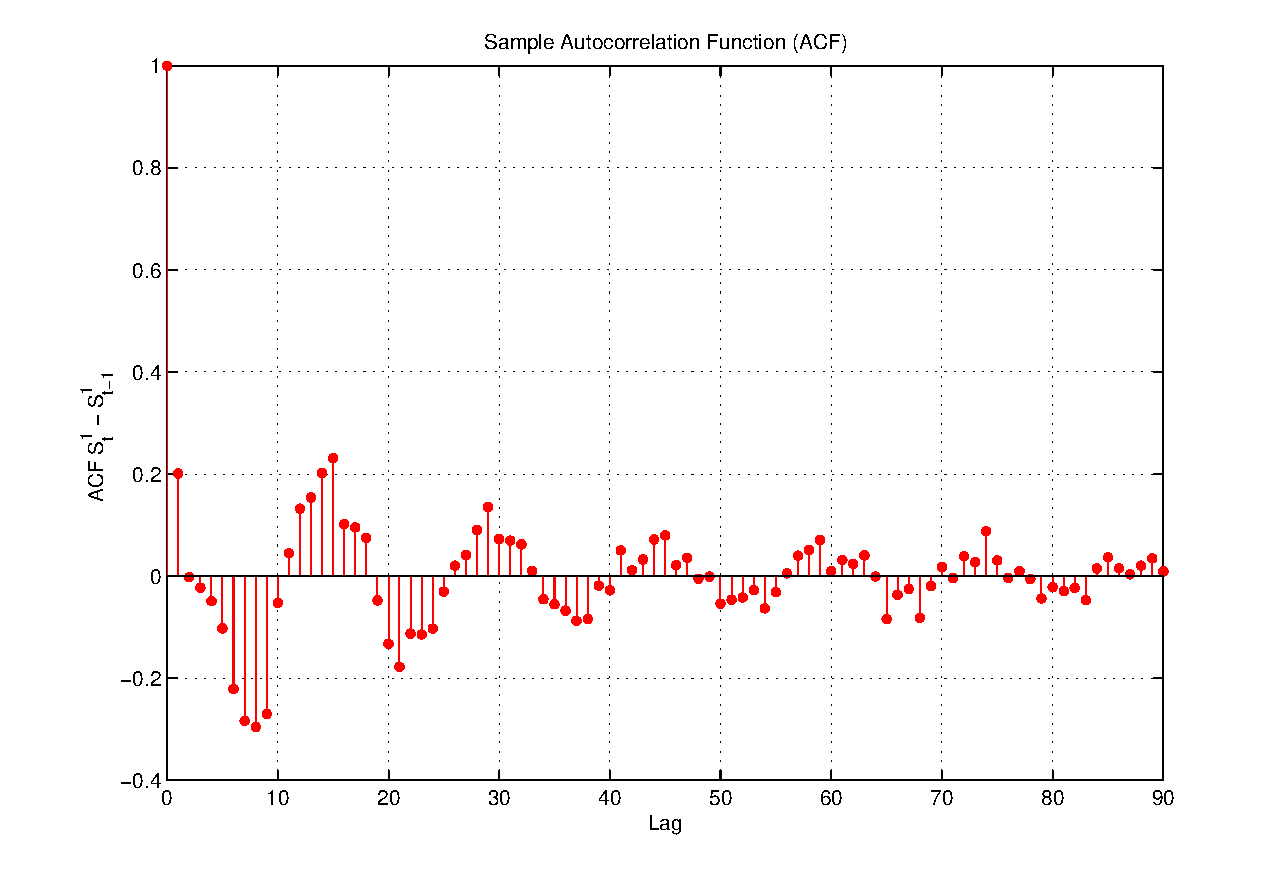
\includegraphics[width=1.00\textwidth]{../graphics/acfS1.pdf}}}
      \quad
      \subfigure[Autocorrelation of absolute returns of asset 1]{\scalebox{0.33}{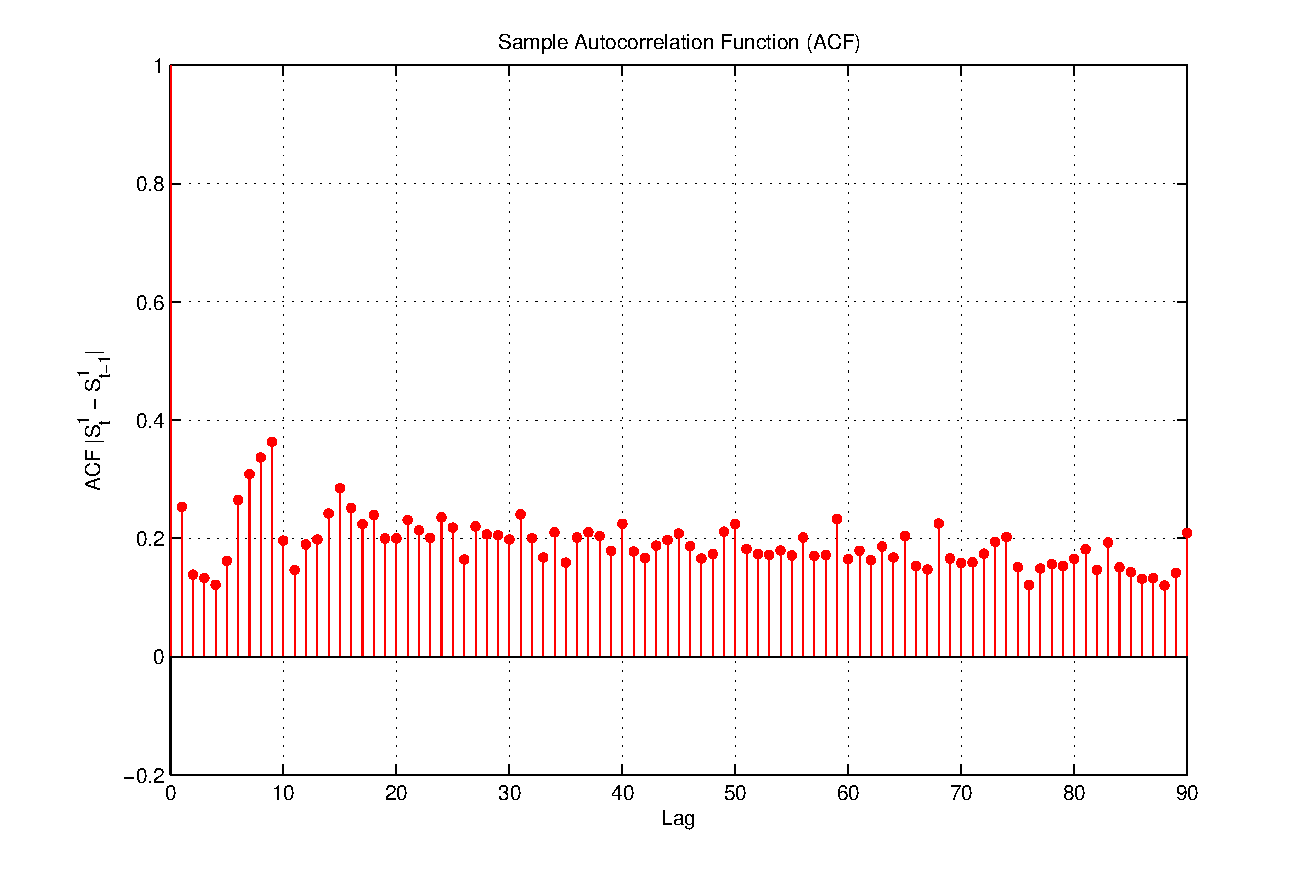
\includegraphics[width=1.00\textwidth]{../graphics/acfabsS1.pdf}}}
      }
    \caption{Examples of outputs and statistics from a single run of the Westerhoff simulation with $K = 5$, $N=0.0002$, $a^M=0.1$, $a^c, b^c = 5$, $a^F, b^F = 0.2$, $f = 1,000,000$ and $g = 1.2$.}
    \label{fig:Westerhoffsim}
  \end{center}
\end{figure}

\section{Verification of Correctness}

The supreme objective was to recreate results reported by others rather than to create a standalone model of the market. Therefore, the validation focused on comparing outputs from our simulations to graphs and statistics from other papers. These compare well with data shown in the original paper (shown in Figures \ref{fig:ContSmallSPap} and \ref{fig:ContLargeSPap}).


\begin{figure}[htbp]
  \begin{center}
    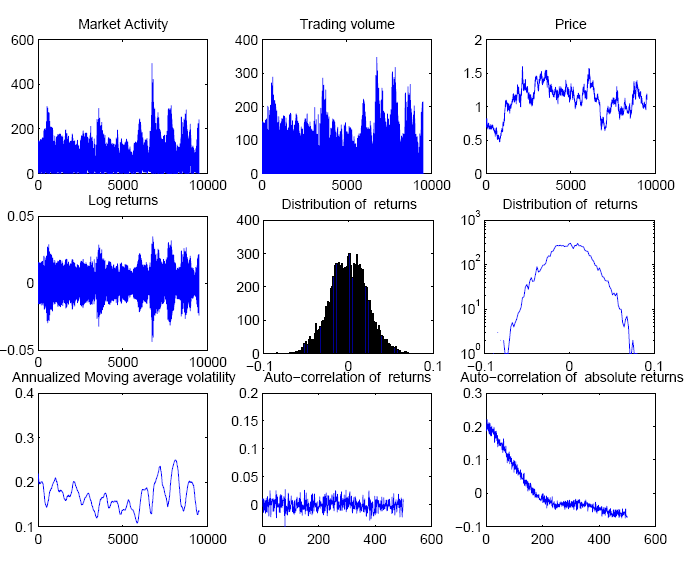
\includegraphics[width=0.8\textwidth]{../graphics/Cont-Fig3.png}
    \caption{Outputs from Cont's paper with $D=0.001$, $s=0.01$. Compare directly to Figure \ref{fig:ContSmallSSim}.}
    \label{fig:ContSmallSPap}
  \end{center}
\end{figure}

\begin{figure}[htbp]
  \begin{center}
    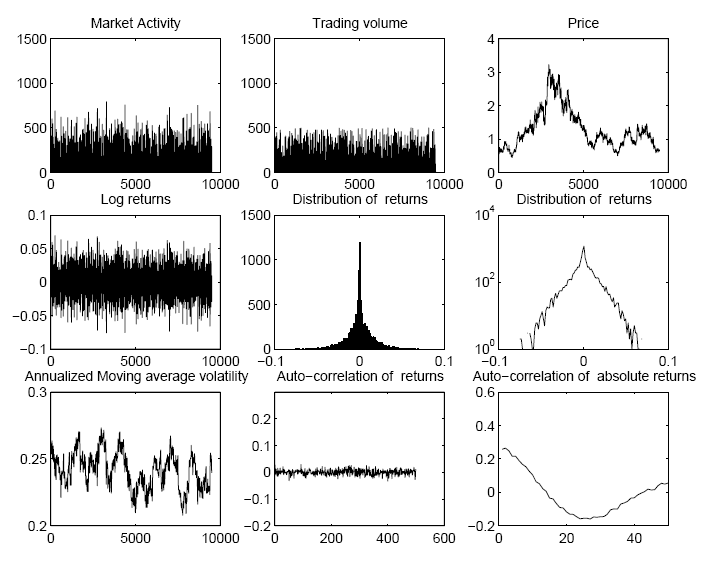
\includegraphics[width=0.8\textwidth]{../graphics/Cont-Fig4.png}
    \caption{Outputs from Cont's paper with $D=0.001$, $s=0.1$. Compare directly to Figure \ref{fig:ContLargeSSim}.}
    \label{fig:ContLargeSPap}
  \end{center}
\end{figure}

\section{Batch Mode Instrumentation}

FinancialMarketModel includes a set of wrappers that are useful for conducting multi-run batch parameter space exploration or sensitivity analysis. A simple wrapper is included in \texttt{experiments} package. Post-run analysis can be performed by using Matlab, sample scripts are included in scripts folder and can be used to render shape of autocorrelation curves and histograms of returns as a function of simulation settings. Figure \ref{fig:ContMultiRun} presents a sample prepared by varying the $D$ news process variance for Cont's model.    


\begin{figure}[htbp]
  \begin{center}
   \mbox{
      \subfigure[Autocorrelation functions]{\scalebox{0.45}{\quad \quad 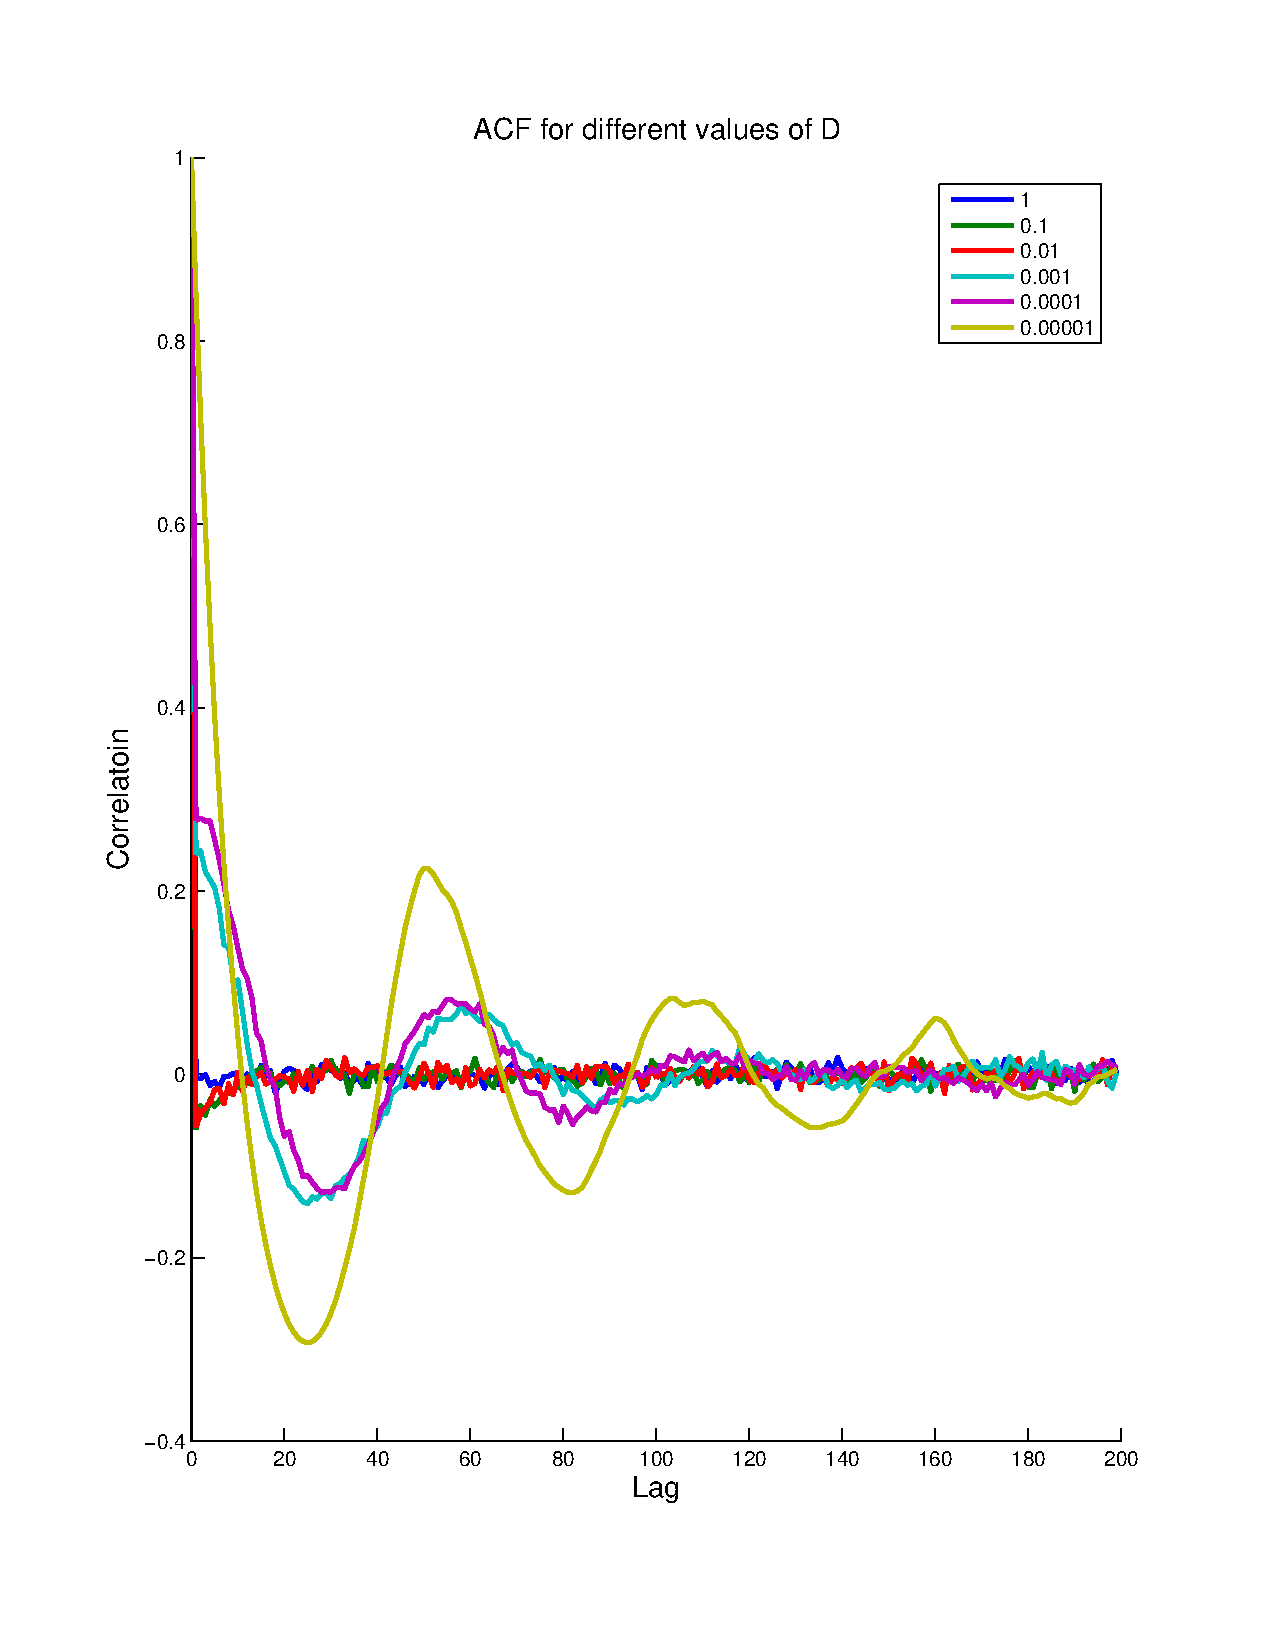
\includegraphics[width=1.0\textwidth]{../graphics/comparisonOfACFs.pdf}}} \quad
      \subfigure[Return distributions]{\scalebox{0.45}{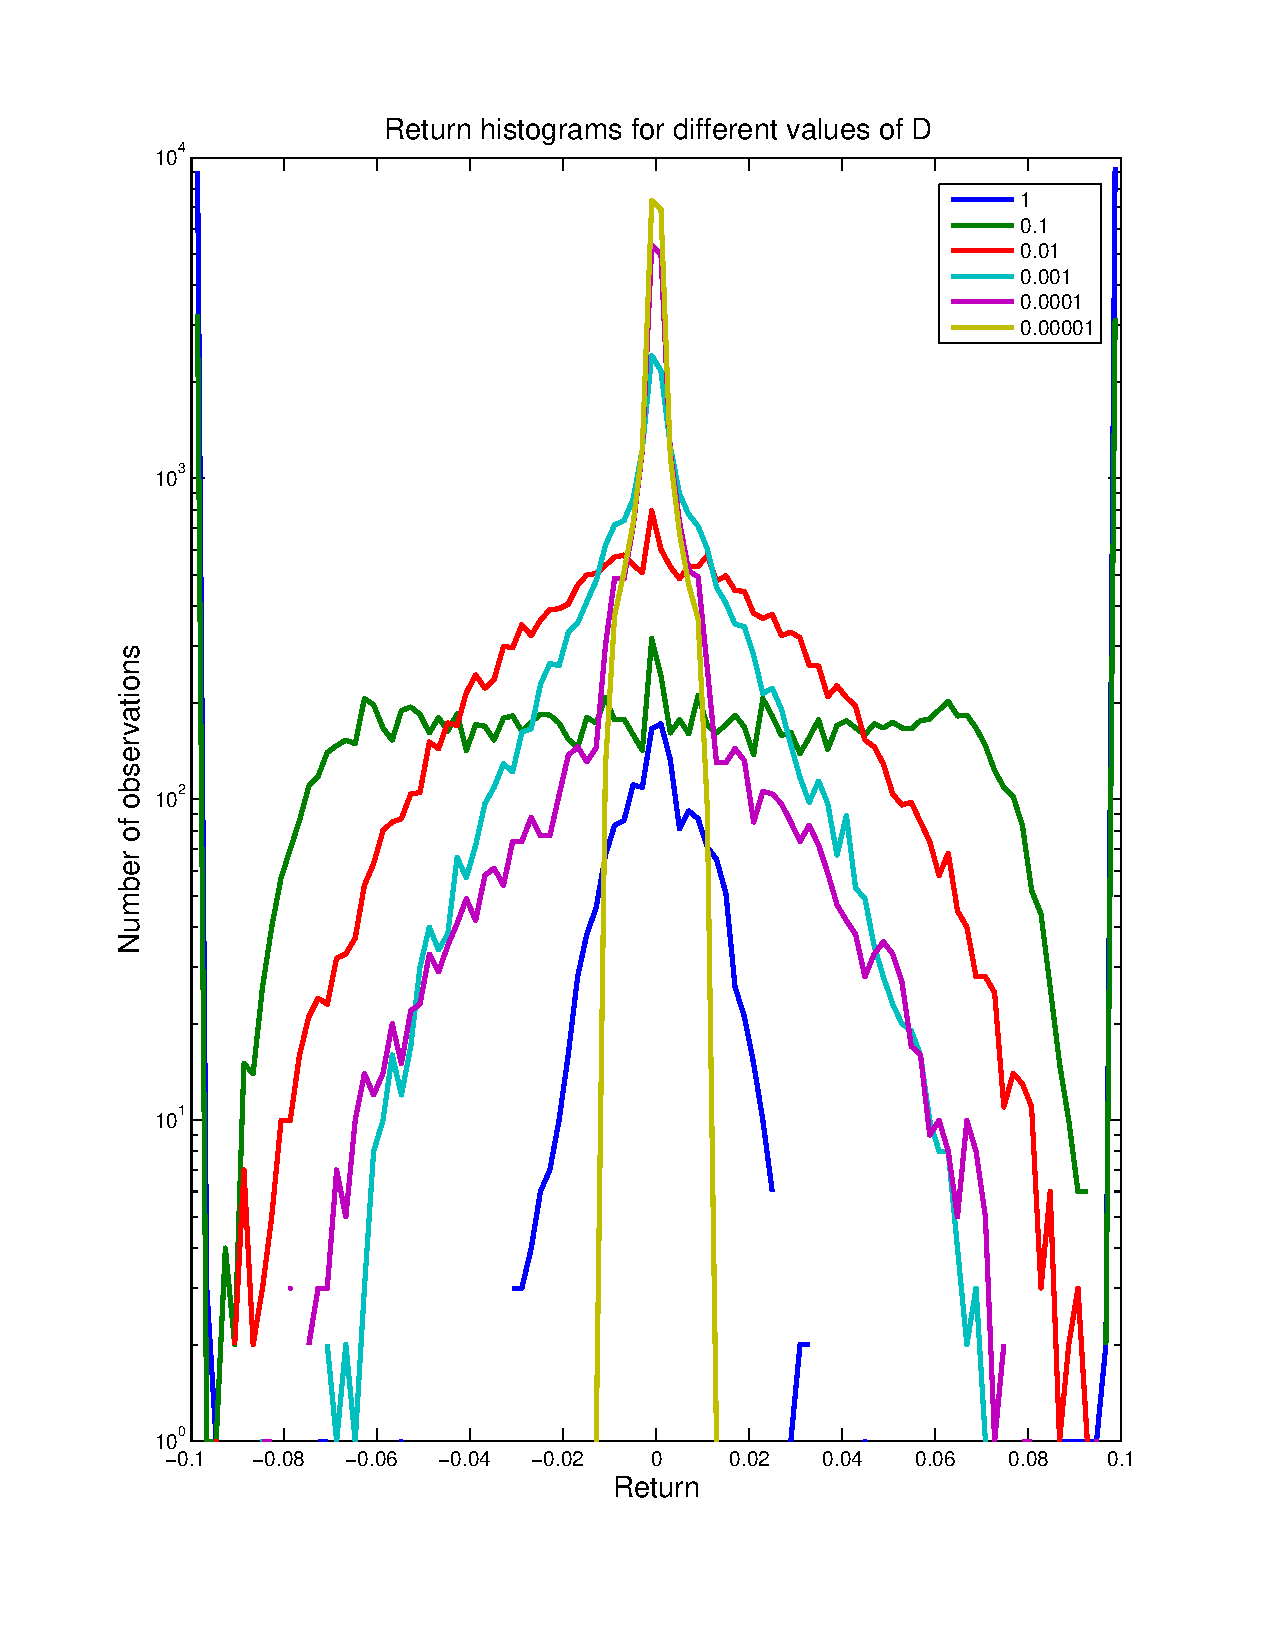
\includegraphics[width=1.00\textwidth]{../graphics/comparisonOfHistograms.pdf}}}
      }
      

      \subfigure[Hurst exponents for different $s$]{\scalebox{0.5}{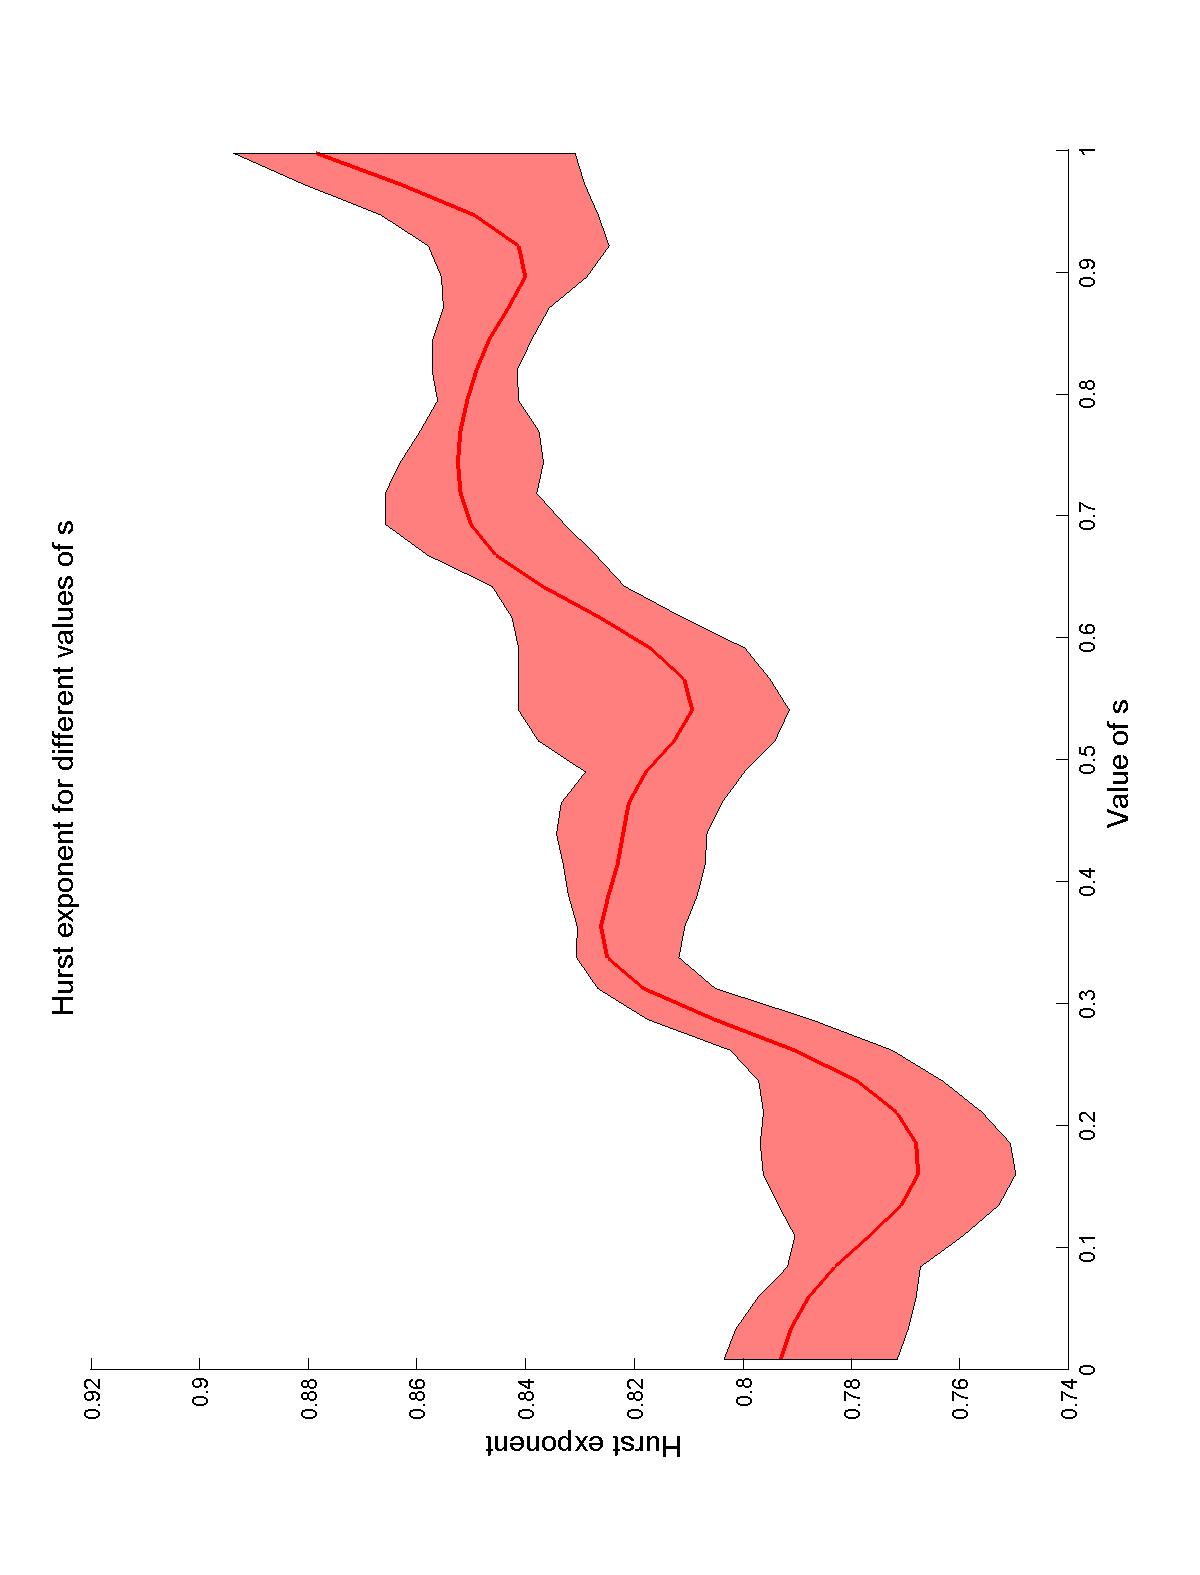
\includegraphics[width=0.9\textwidth, angle=270]{../graphics/comparisonOfHurstsS}}} 
      \subfigure[Hurst exponents for different $D$]{\scalebox{0.5}{\includegraphics[width=0.9\textwidth, angle=270]{../graphics/comparisonOfHurstsD}}}

    \caption{Autocorrelation and distributions in Cont simulation with $s=0.1$ and varying $D$, averaged over many runs. In bottom row, kernel regresion with 95\% resampled confidence intervals on Hurst exponents of time series generated from Con't model for varying levels of $s$ and $D$ is presented.}
    \label{fig:ContMultiRun}
  \end{center}
\end{figure}

\bibliographystyle{plainnat}
\bibliography{master}

\end{document}

%%%%%%%%%%%%%%%%%%%%%%%%%%%%%%%%%%%%%%%%%%%%%%%%%%%%%%%%%%%%%%%%%%%%%%
%% The end.
%%%%%%%%%%%%%%%%%%%%%%%%%%%%%%%%%%%%%%%%%%%%%%%%%%%%%%%%%%%%%%%%%%%%%% 
